%%%%%%%%%%%%%%%%%%%%%%%%%%%%%%%%%%%%%%%%%
% Journal Article
% LaTeX Template
% Version 1.4 (15/5/16)
%
% This template has been downloaded from:
% http://www.LaTeXTemplates.com
%
% Original author:
% Frits Wenneker (http://www.howtotex.com) with extensive modifications by
%  - Vel (vel@LaTeXTemplates.com)

%  - Alejandro M. Aragón (a.m.aragon@tudelft.nl)
%
% License:
% CC BY-NC-SA 3.0 (http://creativecommons.org/licenses/by-nc-sa/3.0/)
%
%%%%%%%%%%%%%%%%%%%%%%%%%%%%%%%%%%%%%%%%%

%----------------------------------------------------------------------------------------
%	PACKAGES AND OTHER DOCUMENT CONFIGURATIONS
%----------------------------------------------------------------------------------------

\documentclass[twoside,twocolumn,10pt]{article}

\usepackage{blindtext} % Package to generate dummy text throughout this template 

\usepackage[sc]{mathpazo} % Use the Palatino font
\usepackage[T1]{fontenc} % Use 8-bit encoding that has 256 glyphs
\linespread{1.05} % Line spacing - Palatino needs more space between lines
\usepackage{microtype} % Slightly tweak font spacing for aesthetics
\usepackage[english]{babel} % Language hyphenation and typographical rules
\usepackage{graphicx}
\usepackage{physics}
\usepackage{amsmath, amssymb}


\usepackage[hmarginratio=1:1,top=25mm,left=20mm,right=20mm,bottom=25mm,columnsep=20pt]{geometry} % Document margins
\usepackage[hang, small,labelfont=bf,up,textfont=it,up]{caption} % Custom captions under/above floats in tables or figures
\usepackage{booktabs} % Horizontal rules in tables

\usepackage{lettrine} % The lettrine is the first enlarged letter at the beginning of the text

\usepackage{enumitem} % Customized lists
\setlist[itemize]{noitemsep} % Make itemize lists more compact

\usepackage{abstract} % Allows abstract customization
\renewcommand{\abstractnamefont}{\normalfont\bfseries} % Set the "Abstract" text to bold
\renewcommand{\abstracttextfont}{\normalfont\small\itshape} % Set the abstract itself to small italic text

\usepackage{titlesec} % Allows customization of titles
\renewcommand\thesection{\Roman{section}} % Roman numerals for the sections
\renewcommand\thesubsection{\roman{subsection}} % roman numerals for subsections
\titleformat{\section}[block]{\large\scshape\centering}{\thesection.}{1em}{} % Change the look of the section titles
\titleformat{\subsection}[block]{\large}{\thesubsection.}{1em}{} % Change the look of the section titles
\usepackage{float}

\usepackage{fancyhdr} % Headers and footers
\pagestyle{fancy} % All pages have headers and footers
\fancyhead{} % Blank out the default header
\fancyfoot{} % Blank out the default footer
\fancyhead[C]{Final Project for Advanced FEM (ME46050) $\bullet$ Aug 2023 $\bullet$ Vol. XXI, No. 1} % Custom header text
\fancyfoot[RO,LE]{\thepage} % Custom footer text

\usepackage{titling} % Customizing the title section


\usepackage[dvipsnames, table]{xcolor}
\usepackage{booktabs}
\usepackage{tabularx}
\usepackage{multirow}
\usepackage{threeparttable}
\usepackage{subcaption}
\usepackage{listings}
\lstset{
  basicstyle=\ttfamily\small,  % 设置代码字体和大小
  numbers=left,                % 行号放在左侧
  breaklines=true, % 设置自动换行
  numberstyle=\tiny,          % 行号的字体大小
  keywordstyle=\color{blue},  % 关键字颜色
  commentstyle=\color{green}, % 注释颜色
  stringstyle=\color{red},    % 字符串颜色
  frame=single,               % 代码周围的框
  rulecolor=\color{black},    % 框的颜色
  xleftmargin=2em,            % 代码块左侧的边距
  captionpos=b                % 标题位置在底部
}

\usepackage{hyperref} % For hyperlinks in the PDF
\hypersetup{colorlinks=true, linkcolor=black, filecolor=black, urlcolor=black, citecolor=black}



\newcolumntype{L}[1]{>{\hsize=#1\hsize\raggedright
  \arraybackslash}X}
\newcolumntype{R}[1]{>{\hsize=#1\hsize\raggedleft
  \arraybackslash}X}
\newcolumntype{C}[2]{>{\hsize=#1\hsize\columncolor{#2}
  \centering\arraybackslash}X}
\newcommand{\ra}[1]{\renewcommand{\arraystretch}{#1}}
\newcommand{\scell}[2]{\cellcolor{#2} #1 }


\usepackage{pgfplots}
\usetikzlibrary{calc}
\usepgfplotslibrary{colorbrewer}


%----------------------------------------------------------------------------------------
%	TITLE SECTION
%----------------------------------------------------------------------------------------

\setlength{\droptitle}{-6\baselineskip} % Move the title up

\pretitle{\begin{center}\Huge\bfseries} % Article title formatting
\posttitle{\end{center}} % Article title closing formatting
\title{Final Project for Advanced FEM (ME46050)} % Article title
\author{%
\textsc{Xusen Qin} \\[1ex] % Your name
\normalsize Student ID: 5594979, email \href{X.Qin-2@student.tudelft.nl}{X.Qin-2@student.tudelft.nl}, % Your email address
edition: 2022-2023
}
\date{} % Leave empty to omit a date
\renewcommand{\maketitlehookd}{%
%\begin{abstract}
%\noindent \blindtext % Dummy abstract text - replace \blindtext with your abstract text
%\end{abstract}
}

%----------------------------------------------------------------------------------------

\begin{document}

% Print the title
\maketitle

%----------------------------------------------------------------------------------------
%	ARTICLE CONTENTS
%----------------------------------------------------------------------------------------

\section{Introduction}

\lettrine[nindent=0em,lines=3]{T}his report addresses two advanced finite element problems. The first problem constructs a solver for a one-dimensional Poisson equation using both h-version and p-version finite elements. The second problem develops a solver for a two-dimensional stress distribution of elliptical inhomogeneity in plane elasticity, employing the h-version FEM with T3 elements and Q4 elements.


\section{\textbf{PROBLEM 1}}
\subsection{Question 1}
The definition of the 1-D Poisson equation is in the Appendix.\ref{Apdx:Q1}
The code for finite element method, shape functions as well as the Gaussian integration method in Appendix.\ref{Apdx:FEM_1D}, \ref{Apdx:shape_1D}, and \ref{Apdx:Gaussian-1D}.

\begin{figure}[htbp]
  \centering
  \begin{subfigure}[b]{0.32\textwidth}
    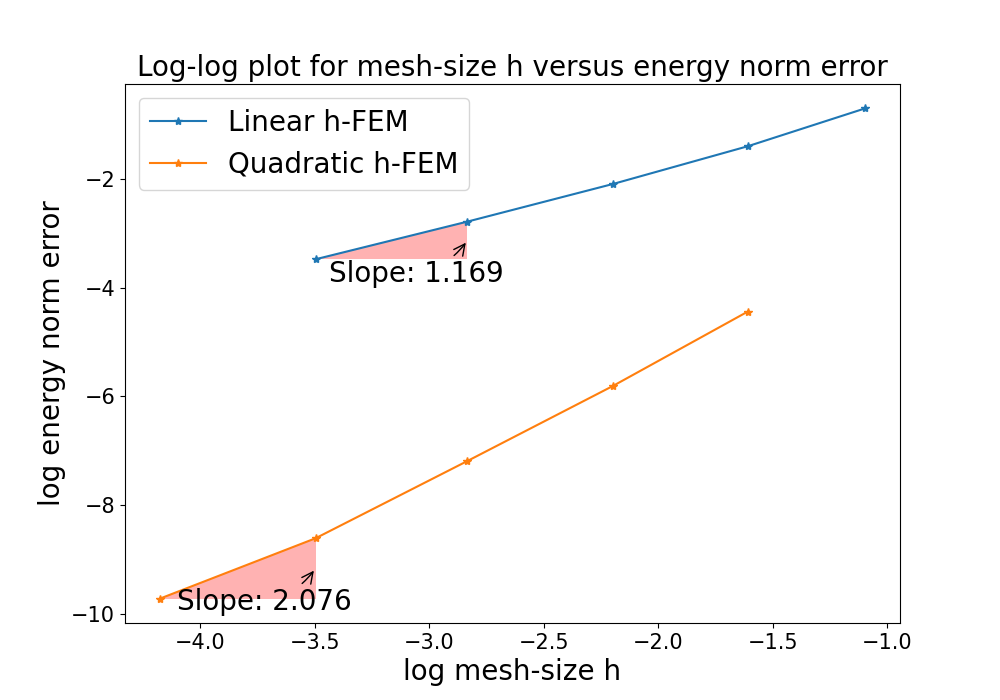
\includegraphics[width=1.\linewidth]{Q1/logmeshsize.png}
    \caption{log-log plot for the error versus meshsize}
    \label{fig:logmeshsize}
  \end{subfigure}
  % \hfill
  \begin{subfigure}[b]{0.32\textwidth}
    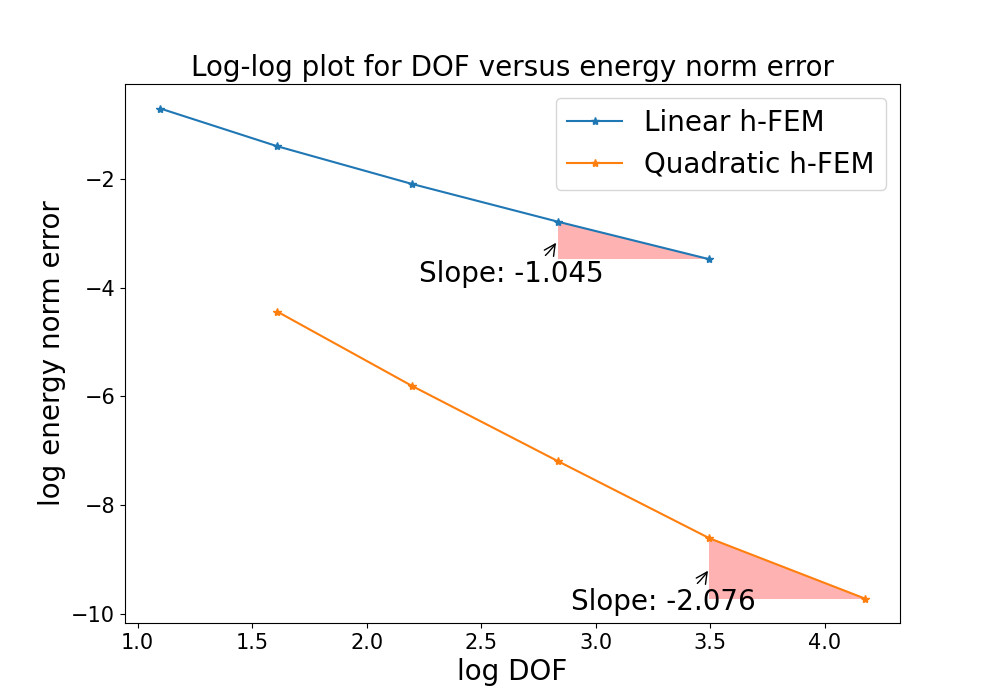
\includegraphics[width=1.\linewidth]{Q1/logDOF.png}
    \caption{log-log plot for the error versus DOF}
    \label{fig:logDOF}
  \end{subfigure}
\caption{The log-log figure for the energy norm error versus mesh size and DOF.}
\label{fig:Q1_1}
\end{figure}

The precise strain energy for this problem is given as U=0.03559183822564316. To determine the rates of convergence in the energy norm for both element types, we focus on terminal convergence by considering the last two points in the convergence plots.

The formula for the convergence rate can be found in Eq.\ref{eq:rate}, which can also be defined as the slope of the log-log plot. The mesh size \( h \) is defined as \( h = \frac{1}{{\text{DOF}}^d} \), where \( d \) is the dimensionality of the problem. In this case, we take \( d = 1 \). For both elements, the error decreases with the increase of the DOFs and the decrease of the mesh size. It's noteworthy that the convergence rate for the quadratic elements is approximately greater than that for the linear elements. Given the smoothness of the solution, the theoretical rates of convergence are typically -1.045 for linear elements and -2.076 for quadratic elements concerned with DOFs, which is equal to the order of the polynomials. For the computed errors, the linear elements exhibit an error of approximately \(0.031\), while the quadratic elements have a significantly smaller error of about \(6.0 \times 10^{-5}\). These computed rates align closely with the theoretical expectations.

\begin{equation}
\text{Rate} = \frac{\log(\text{error}_2) - \log(\text{error}_1)}{\log(\text{DOF}_2) - \log(\text{DOF}_1)}
\label{eq:rate}
\end{equation}

\subsection{Question 2}
In the log-log plot in Fig.\ref{fig:h_p_error} of the relative error in the energy norm versus the number of DOFs, the slopes of the plotted lines represent these rates. The following items are observed.

\begin{itemize}
    \item For Linear h-FEM: The rate of convergence is approximately -1.045.
    \item For Quadratic h-FEM: The rate of convergence is approximately -2.076.
    \item For p-FEM: The rate of convergence is approximately -8.230.
\end{itemize}
The negative values for the convergence rates indicate that the error decreases as the number of DOFs increases, which is expected in a convergence study. Notably, the rate of convergence of the linear element is close to 1, and the quadratic element is close to 2, respectively, which indicates that the convergence rate of h-FEM is equal to the polynomial order. From the rates, it's evident that the p-FEM has the steepest convergence, indicating a faster reduction in error with increasing DOFs compared to the other methods. 

\begin{figure}[!ht]
  \centering
  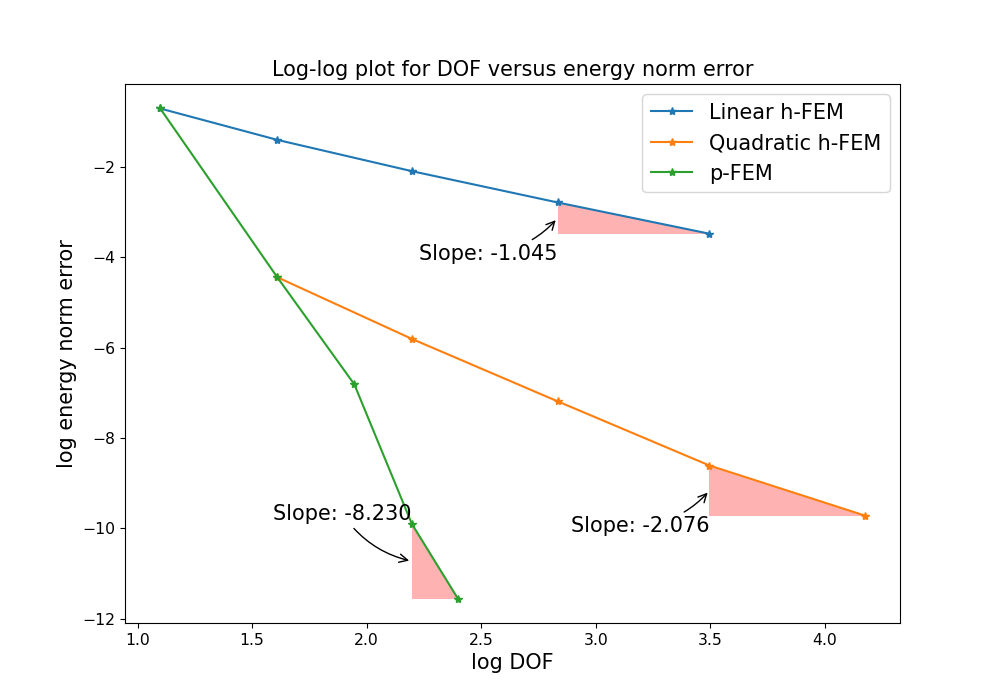
\includegraphics[width=1.\linewidth]{Q1/h_p_error.png}
  \caption{ log-log plot of the error versus DOF in h-version and p-version FEM.}
  \label{fig:h_p_error}
\end{figure}

\subsection{Question 3}

In order to estimate the error in finite element method solutions, we use a posteriori error analysis based on the energy norms described in the following processes.

Considering the algebraic convergence of the energy norm error for exact solution $u$ and the finite elements solution $u_h$ in energy space $\epsilon(\Omega)$:

\begin{equation}
  \left\|u-u^h\right\|_{\epsilon(\Omega)} \leqslant C_1 h^{\beta_h}\|u\|_{\epsilon(\Omega)}
\end{equation}

We went:

\begin{equation}
 \|u\|_{\epsilon(\Omega)} = \sqrt{U}
\end{equation}
where $U$ is the exact strain energy.

Considering the relation between the energy and binary term in the finite element methods.

\begin{equation}
  \begin{aligned}
  u(u) &= \frac{1}{2} B(u, u), \\
  \|u\|_e &= \sqrt{\frac{1}{2} B(u, u)}, \\
  \|u-u^h\|_e &= \frac{1}{2} B\left(u-u^h, u-u^h\right) \\
  &= \frac{1}{2} B(u, u) - \frac{1}{2} B\left(u^h, u^h\right), \\
\end{aligned}
\end{equation}

Now we obtain the error of the strain energy:

\begin{equation}
  \begin{aligned}
U_e &= U - U^h.
\end{aligned}
\end{equation}

By using the energy values obtained from three different mesh sizes, a system of equations can be constructed to determine the exact solution 
$U$:
\begin{equation}
\begin{aligned}
  & U-U^{h_0}=C_1^2 h_0^{2 \beta_h} U \, \text{(I)}\\
  & U-U^{h_1}=C_1^2 h_1^{2 \beta_h} U \, \text{(II)}\\
  & U-U^{h_2}=C_1^2 h_2^{2 \beta_h} U \, \text{(III)}
\end{aligned}
\label{eq:U_h}
\end{equation}

In these equations:
\begin{itemize}
    \item \( U^{h_0} \), \( U^{h_1} \), and \( U^{h_2} \) are the FEM approximated solutions for mesh sizes \( h_0 \), \( h_1 \), and \( h_2 \) respectively.
    \item \( C_1 \) is a coefficient.
    \item \( \beta_h\) is an exponent that determines the convergence rate of error reduction as mesh size decreases.
\end{itemize}

The logarithmic relationship between the errors for different mesh sizes can be obtained obtained by Eq.\ref{eq:U_h}:

\begin{equation}
\begin{aligned}
  \text{Take } \frac{\log(\text{I})}{\log(\text{II})} & : \log \left( \frac{U-U^{h_0}}{U-U^{h_1}} \right) = 2 \beta_h \log \left(\frac{h_0}{h_1}\right) \\
  \text{Take } \frac{\log(\text{II})}{\log(\text{III})} & : \log \left( \frac{U-U^{h_1}}{U-U^{h_2}} \right) = 2 \beta_h \log \left(\frac{h_1}{h_2}\right) \\
\end{aligned}
\label{eq:logU_h} 
\end{equation}

These equations provide insight into how the error changes logarithmically as the mesh size changes.

Using the above relationships, the a posteriori error estimate, which is a measure of the relative error, is expressed as:

\begin{equation}
\frac{\log \left( \frac{U-U^{h_0}}{U-U^{h_1}} \right)}{\log \left( \frac{U-U^{h_1}}{U-U^{h_2}} \right)} = \frac{\log \left( \frac{h_0}{h_1} \right)}{\log \left( \frac{h_1}{h_2} \right)} = \textbf{Q}
\label{eq:Q_relation}
\end{equation}

Considering the relation between the mesh size $h$ and the $DOF$ ($N$):

\begin{equation}
 h \cong \frac{1}{N^{1 / dimensionality}}
\end{equation}

The expression of $\textbf{Q}$ is given by:

\begin{equation}
  Q=\frac{\log \left(N_1 / N_0\right)}{\log \left(N_2 / N_1\right)}
\end{equation}

The term \( \textbf{Q} \) gives a weighted comparison of the errors between different mesh sizes. This relationship becomes pivotal in understanding the error behavior across different mesh sizes.

By repeatedly applying the aforementioned process for multiple mesh sizes and averaging the computed energies, a more accurate representation of the solution's energy is achieved, which provides a reliable posterior error estimate.

\begin{table}[!ht]
  \centering
  \begin{tabular}{|l|c|c|}
      \hline
      & \textbf{Energy} & \textbf{Relative Error} \\
      \hline
      Linear & 0.034626674 & 2.7117($\%$) \\
      \hline
      Quadratic & 0.035591726 & 0.000314($\%$) \\
      \hline
      Exact solution & 0.035591838 & $/$ \\
      \hline
  \end{tabular}
  \caption{Energy obtained by a posterior estimate and Relative Error values for different FEM methods}
  \label{tab:fem_values}
\end{table}

 As shown in the table.\ref{tab:fem_values}, for the linear FEM, the energy is computed to be \(0.03463\), which results in a relative error of \(2.7117\%\). This indicates a slight deviation from the exact solution. On the other hand, the quadratic FEM provides an energy value of \(0.03559\), which is extremely close to the exact solution with a minuscule relative error of \(0.000314\%\). This suggests that the quadratic FEM is significantly more accurate than the linear FEM for this problem. 

In summary, while the linear FEM offers a reasonable approximation, the quadratic FEM provides an almost exact match to the true solution in terms of energy.

The code for a posterior estimate is provided in the Appendix.\ref{Apdx:post}.

\subsection{Question 4}
In the h-version study using the quadratic finite element method, we analyzed the model with varying mesh sizes, namely 5, 10, 20, and 40 evenly spaced elements. Fig.\ref{fig:q_4} represents the h-FEM solutions with four mesh sizes. A comparison of the numerical solutions against the exact solution provided insights into the accuracy of the employed method. From Fig.\ref{fig:h_error_4} it was discernible that the graph wasn't strictly linear. However, by focusing on the terminal two data points, we derived an asymptotic rate of convergence of \(-2.122\). This suggests a quadratic rate of reduction in error relative to the refinement in element size. For this specific problem, the exact strain energy is given by \( U = 1.585854059271320 \), and the computed results $U_{FEM} = 1.5845186616720888$ is close to this value.  

\begin{figure}[!ht]
  \centering
  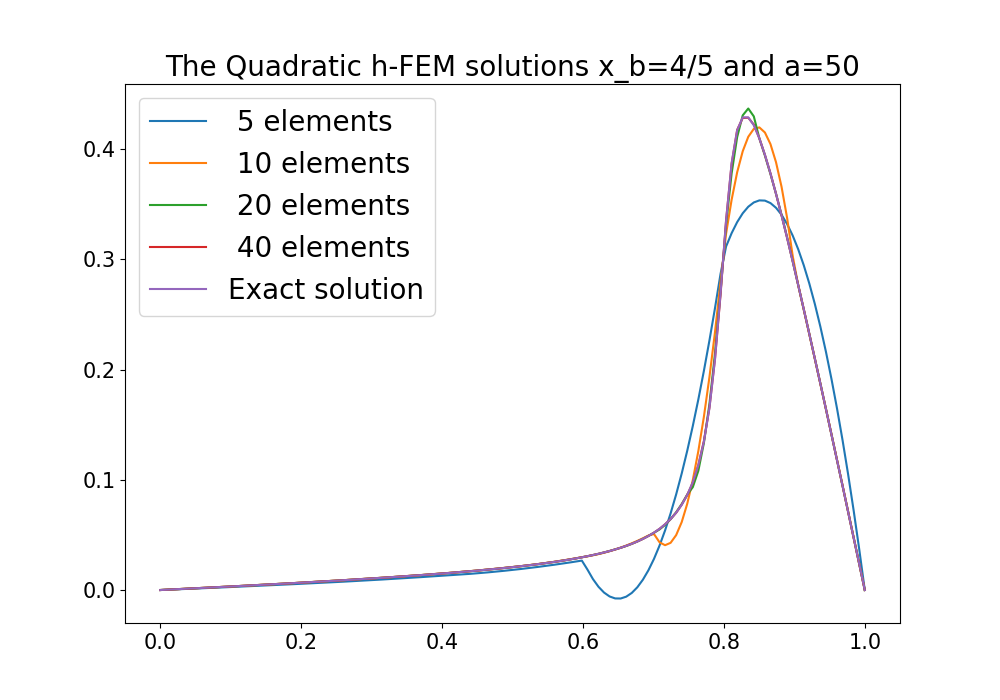
\includegraphics[width=1.\linewidth]{Q1/Q1_4.png}
  \caption{The Quadratic h-FEM solutions $x_b$=4/5 and $a$=50 with different element numbers.}
  \label{fig:q_4}
\end{figure}

\begin{figure}[!ht]
  \centering
  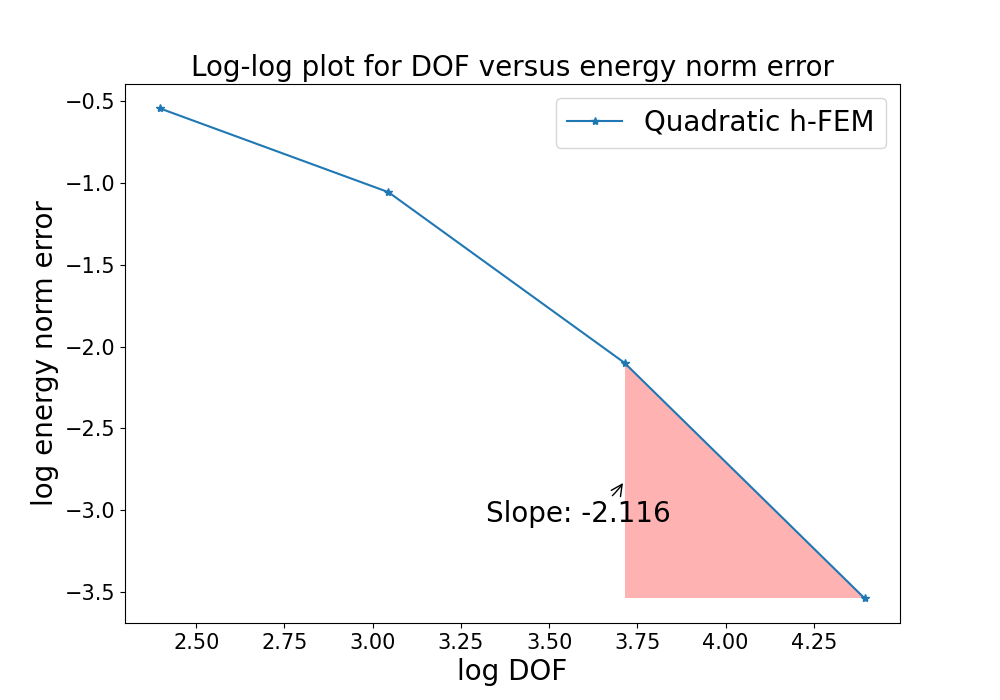
\includegraphics[width=1.\linewidth]{Q1/logDOF_q_4.png}
  \caption{Log-log plot for DOF versus energy norm error.}
  \label{fig:h_error_4}
\end{figure}

\subsection{Question 5}
% In the p-version study, the problem was analyzed using 5 elements with polynomial degrees ranging from \( p = 1 \) to \( p = 5 \). The numerical solutions obtained were juxtaposed against the exact solution, providing a comprehensive understanding of the precision of our approach, as depicted in Fig.\ref{fig:p_5}. Further insights were gleaned from the log-log plot showcasing the relative error in the energy norm against the number of DOFs, illustrated  

From the log-log plot in Fig.\ref{fig:h_p_error_5}, the computed rate of convergence for the p-version was approximately \(-4.882\), whereas for the h-version, it was \(-2.2122\). The convergence rate of quadratic p-FEM is faster than h-FEM in this problem.  As a result, the p-FEM can achieve higher accuracy with fewer degrees of freedom.

\begin{figure}[!ht]
  \centering
  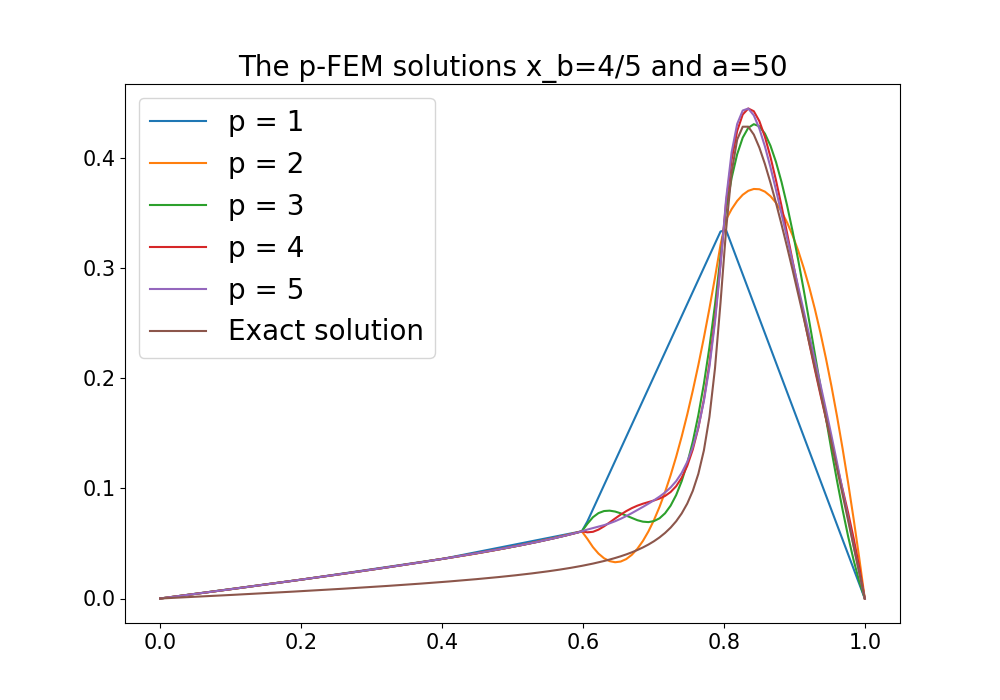
\includegraphics[width=1.\linewidth]{Q1/Q1_5.png}
  \caption{The p-FEM solutions $x_b$=4/5 and $a$=50 with different element numbers.}
  \label{fig:p_5}
\end{figure}

\begin{figure}[!ht]
  \centering
  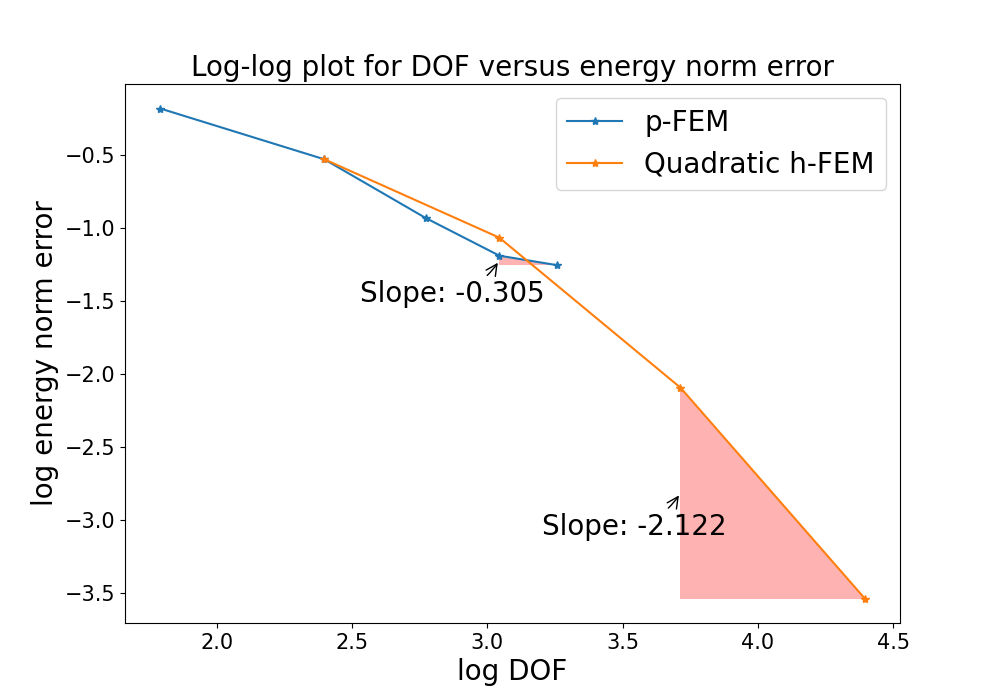
\includegraphics[width=1.\linewidth]{Q1/h_p_error_5.png}
  \caption{Log-log plot for DOF versus energy norm error in p-FEM and h-FEM.}
  \label{fig:h_p_error_5}
\end{figure}

\subsection{Question 6}

The stability of numerical methods in finite element analysis can be assessed using the condition number of the stiffness matrix.

Observing the log-log plot in Fig.\ref{fig:contK}:
\begin{itemize}
    \item \textbf{p-FEM}: The condition number remains constant regardless of the DOFs increase, indicating its robustness.
    
    \item \textbf{Quadratic h-FEM}: Condition number growth is consistent with increasing DOFs and is unaffected by equation parameter changes (both for \(a=0.5\) and \(a=50\)).
    
    \item \textbf{Linear vs Quadratic h-FEM}: Both show similar growth trends, but the linear version has a slightly lower condition number for similar DOFs.
\end{itemize}

In summary, p-FEM stands out in stability, while h-FEM versions show predictable growth trends, with the linear version in slightly better condition.



\begin{figure}[!ht]
  \centering
  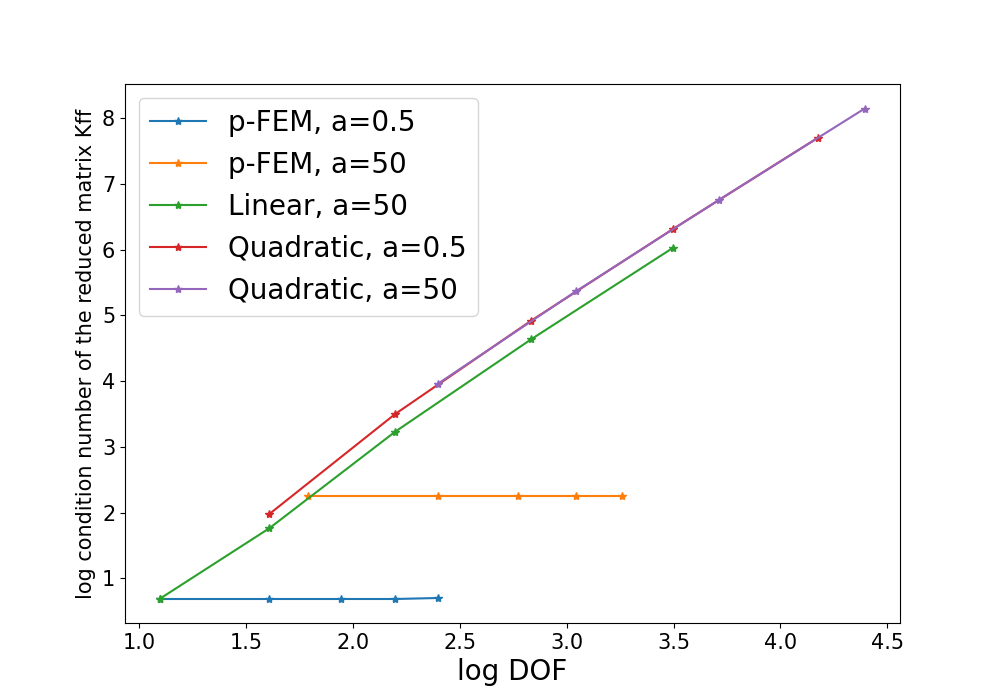
\includegraphics[width=1.\linewidth]{Q1/cont_K.png}
  \caption{Log-log plot for the condition number of the reduced matrix $K_{ff}$ versus energy norm error.}
  \label{fig:contK}
\end{figure}

\subsection{Question 7}

\subsubsection{Comparison of Results and Conclusions on Strong Gradients}
From the results obtained, several conclusions can be drawn regarding the behavior of the finite element methods under study, especially in problems with strong gradients or sharp features.

\begin{itemize}
    \item \textbf{Convergence Rate and Accuracy}: The convergence rate, represented as the slope of the log-log plot, provides insights into the efficacy of the different finite element methods. The error decreased with the increase of the DOFs and the decrease of the mesh size. Notably, the quadratic elements exhibited a more significant convergence rate than the linear ones, reflecting the theoretical expectations. Meanwhile, the rate of convergence for h-FEM is equal to the polynomial order.
    
    \item \textbf{Linear h-version}: For the linear FEM, the energy was computed to be somewhat deviated from the exact solution, especially in problems with sharp features. This indicates that while the linear h-FEM offers a reasonable approximation, there's a clear margin for improvement in accuracy for such problems.
    
    \item \textbf{Quadratic h-version}: In sharp gradient problems, the quadratic h-FEM showed its strength by providing an energy value that was extremely close to the exact solution, emphasizing its higher accuracy.
    
    \item \textbf{p-version vs. h-version in Sharp Problems}: In problems with sharp gradients, the p-version exhibited remarkable resilience and adaptability. Despite its slower convergence rate, it outperformed both the linear and quadratic h-versions in terms of accuracy for comparable DOFs. This suggests that the p-version, with its adaptability, can better capture local variations and sharp features without requiring extensive mesh refinements that h-version methods might demand.
    
    \item \textbf{Effect of Strong Gradients}: The p-FEM is particularly effective for problems with strong gradients or sharp features. Its higher-order polynomial approximations and local refinement capabilities allow it to capture complex variations in the solution more accurately than methods like h-FEM. This adaptability often results in higher accuracy with fewer computational resources.

    
    \item \textbf{Stability and Robustness}: The stability of finite element methods, assessed by the condition number of the stiffness matrix, highlighted the robustness of the p-FEM. Its condition number remains invariant with increasing DOFs, ensuring consistent performance. On the other hand, the h-FEM versions, both linear and quadratic, exhibit predictable growth in condition numbers, with the linear version showing a slight edge in conditioning. The quadratic h-FEM's stability remains consistent even with changes in equation parameters.
    
\end{itemize}

\subsubsection{Quadrature Points and Computation Efficiency}
In p-FEM, higher-order shape functions demand precise integral evaluations, achieved effectively with Gauss quadrature. Given the complexity of these functions, 9 Gauss points were selected to ensure accurate integration of non-linear shape functions. While more Gauss points increase precision, they also require more computational effort. As is shown in Fig.\ref{fig:h_p_error_5_6}, when setting the Gaussian point as 6, the result of p-FEM cannot represent the convergence well in a strong gradient problem.

\begin{figure}[!ht]
  \centering
  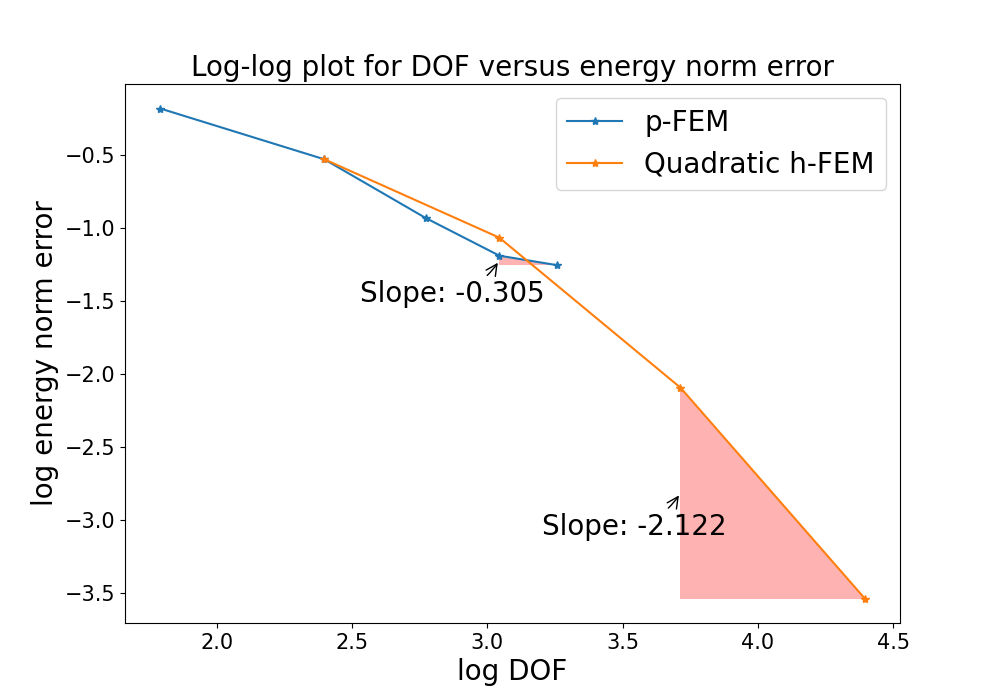
\includegraphics[width=1.\linewidth]{Q1/h_p_error_5_3.png}
  \caption{Log-log plot for DOF versus energy norm error in p-FEM and h-FEM when Gaussian points are selected as 6.}
  \label{fig:h_p_error_5_6}
\end{figure}

\section{\textbf{PROBLEM 2}}
\subsection{Questions 1}
The definition of the traction-free hole in an infinite plate with different a/b ratios is shown in Appendix.\ref{Apdx:Q2} of the report.
 The code for finite element method, shape functions as well as the Gaussian integration method in Appendix.\ref{Apdx:FEM_2D}, \ref{Apdx:shape_2D}, and \ref{Apdx:Gaussian_2D}. For the mesh size $h/L=0.05$ and Q4 mesh, the displacement fields for different a/b are represented in Fig.\ref{fig:disp}.

\begin{figure}[!ht]
  \centering
  \begin{subfigure}[c]{0.32\textwidth}
    \centering
    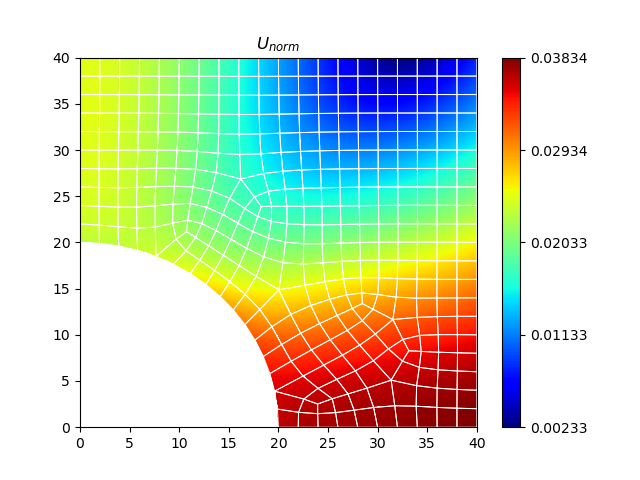
\includegraphics[width=1.\linewidth]{Q2_1/Q1_1_2_quad.png}
    \caption{Displacement field for a/b=1}
    \label{fig:disp_1}
  \end{subfigure} 
  \hfill
  \begin{subfigure}[c]{0.32\textwidth}
    \centering
    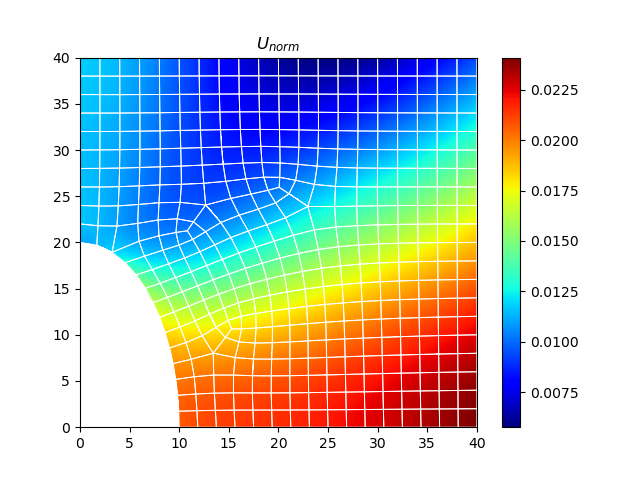
\includegraphics[width=1.\linewidth]{Q2_1/Q1_0.5_2_quad.png}
    \caption{Displacement field for a/b=0.5}
    \label{fig:disp_05}
  \end{subfigure}
  \hfill
  \begin{subfigure}[c]{0.32\textwidth}
    \centering
    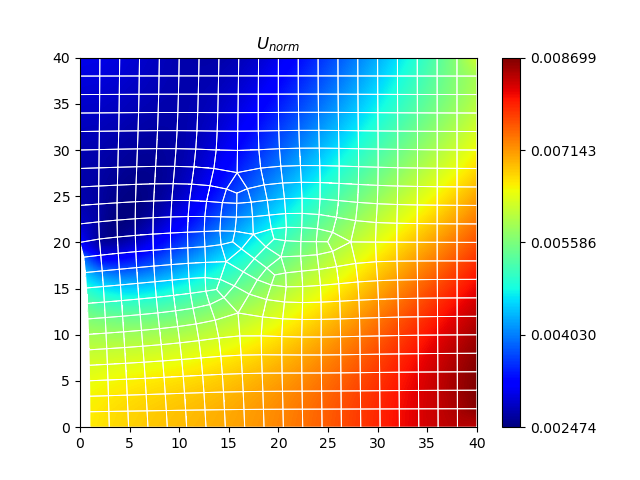
\includegraphics[width=1.\linewidth]{Q2_1/Q1_0.05_2_quad.png}
    \caption{Displacement field for a/b=0.05}
    \label{fig:disp_005}
  \end{subfigure}
  \caption{ displacement fields for different a/b : (a) a/b=1; (b) a/b=0.5; and (c) a/b=0.05.}
  \label{fig:disp}  
\end{figure} 

\subsection{Question 2}

The accurate stress solution at each point is computed using the given formula \cite{jin2014solution}. This is then multiplied by the inverse of the stiffness matrix \(C\) in plain stress assumption, which is given by:

\begin{equation}
C = \frac{E}{1 - \nu^2} \begin{pmatrix}
    1 & \nu & 0 \\
    \nu & 1 & 0 \\
    0 & 0 & \frac{1-\nu}{2}
\end{pmatrix}
\end{equation}

to obtain the strain at each point. Due to the presence of an ellipse in the middle of the plate, the value of the strain at the edge point cannot represent the total strain of the part. Hence, the total strain at the edge points is simplified as the exact strain of the edge point plus the strain at the ellipse vertices:
\[
\epsilon_x(L,0) = \epsilon_x(L,0) + \epsilon_x(a,L),
\]
\[
\epsilon_y(L,0) = \epsilon_y(L,0) + \epsilon_y(L,b).
\]
The displacements are then approximated as \(\text{displacement} = \text{strain} \times 40mm\).

The results and relative error are tabulated in Table.\ref{tab:U_eaxvsfem} and Table.\ref{tab:U_relative_error}.

\begin{table}[h]
\centering
\begin{tabular}{cccccc}
\toprule
a/b ratio & \(U_{x,\text{cal}}\) & \(U_{x,\text{FEM}}\) & \(U_{y,\text{cal}}\) & \(U_{y,\text{FEM}}\) \\
\midrule
1 & 0.01588 & 0.03816 & 0.0004068 & -0.02473  \\
0.5 & 0.01688 & 0.0247 & -0.00484 & -0.01205 \\
0.05 & 0.0176 & 0.01889 & -0.00536 & -0.00658\\
\bottomrule
\end{tabular}
\caption{Computed displacement by simplified assumptions for different a/b ratios }
\label{tab:U_eaxvsfem}
\end{table}

\begin{table}[!ht]
\centering

\begin{tabular}{ccc}
\toprule
a/b ratio & Error in \( U_{x} \) (\%) & Error in \( U_{y} \) (\%) \\
\midrule
1 & 58.39 & 101.64 \\
0.5 & 31.66 & 59.83 \\
0.05 & 6.83 & 18.54 \\
\bottomrule
\end{tabular}
\caption{Relative Errors Between Calculated and FEM-obtained Displacements for Different a/b Ratios}
\label{tab:U_relative_error}
\end{table}

Table \ref{tab:U_relative_error} shows that the relative errors in displacements \( U_{x} \) and \( U_{y} \) decrease as the \( a/b \) ratio diminishes. The highest errors occur at \( a/b = 1 \), reaching up to 101.64\% for \( U_{y} \), suggesting the model's reduced reliability for circular holes. In contrast, the model appears more accurate for narrower ellipses, with errors below 20\% at \( a/b = 0.05 \).


% Considering a plate subjected to plane stress conditions, we assume the following material properties and dimensions:
% \begin{itemize}
%     \item Young's Modulus, \( E = 200 \) GPa.
%     \item Poisson's ratio, \( \nu = 0.3 \).
%     \item Plate thickness, \( h = 1 \) mm.
% \end{itemize}
% Given the applied total force \( P = 2000 \) N and side length \( L = b = 40 \) mm, we aim to estimate the displacements.

% The stress in the x-direction due to the applied force is:
% \begin{equation}
% \sigma_x = \frac{P}{h \times b}
% \end{equation}

% No force in the y-direction implies \( \sigma_y = 0 \).

% The strains in the x and y directions, under plane stress conditions, are:
% \begin{equation}
% \begin{aligned}
% \epsilon_x &= \frac{1}{E} (\sigma_x - \nu \sigma_y) \\
% \epsilon_y &= \frac{1}{E} (\sigma_y - \nu \sigma_x)
% \end{aligned}
% \end{equation}

% Using the strains, the displacements at the boundaries are estimated as:

% \begin{equation}
% \begin{aligned}
% u_x(L, 0) &= \epsilon_x \times L \\
% u_y(0, L) &= \epsilon_y \times L
% \end{aligned}
% \end{equation}

% The estimated displacements at the boundaries are:
% \begin{equation}
% \begin{aligned}
% u_x(L, 0) &\approx 0.01 \, \text{mm} \\
% u_y(0, L) &\approx -0.003 \, \text{mm}
% \end{aligned}
% \end{equation}

% The above displacements are approximations based on plane stress and linear elasticity assumptions.

\subsection{Question 3}

The computed strain energy values for different a/b ratios using different mesh types (T3 and Q4) are presented in Table.\ref{tab:strain_energy_values}. Due to the limitations in calculating the exact strain energy, the computed values from the numerical simulations are considered representative for each mesh type (T3 and Q4). The table shows that the strain energy values vary with the a/b ratio. Specifically, the energy values are highest for a ratio of 1 and decrease as the ratio decreases. This suggests that the structure is more energetically stable when a/b is closer to 1. 

\begin{table}[ht]
\centering
\caption{Computed strain energy values for different a/b ratios (unit kJ).}
\label{tab:strain_energy_values}
\begin{tabular}{cccc}
\toprule
a/b ratio & T3 & Q4 & Average \\
\midrule
1           & 25.898 & 22.337 & 24.1175 \\
0.5         & 17.145 & 18.377 & 17.761 \\
0.05        & 15.449 & 14.443 & 14.946 \\
\bottomrule
\end{tabular}
\end{table}


While we cannot compare these values to the exact strain energy due to computational constraints, the exact strain energy in the following questions is the energy calculated by a posterior error estimate.

\subsection{Question 4}

The log-log plot for energy norm error versus mesh size and DOF are represented in Fig.\ref{fig:logDOF_Q2_4} 
\begin{figure}[!ht]
  \centering
  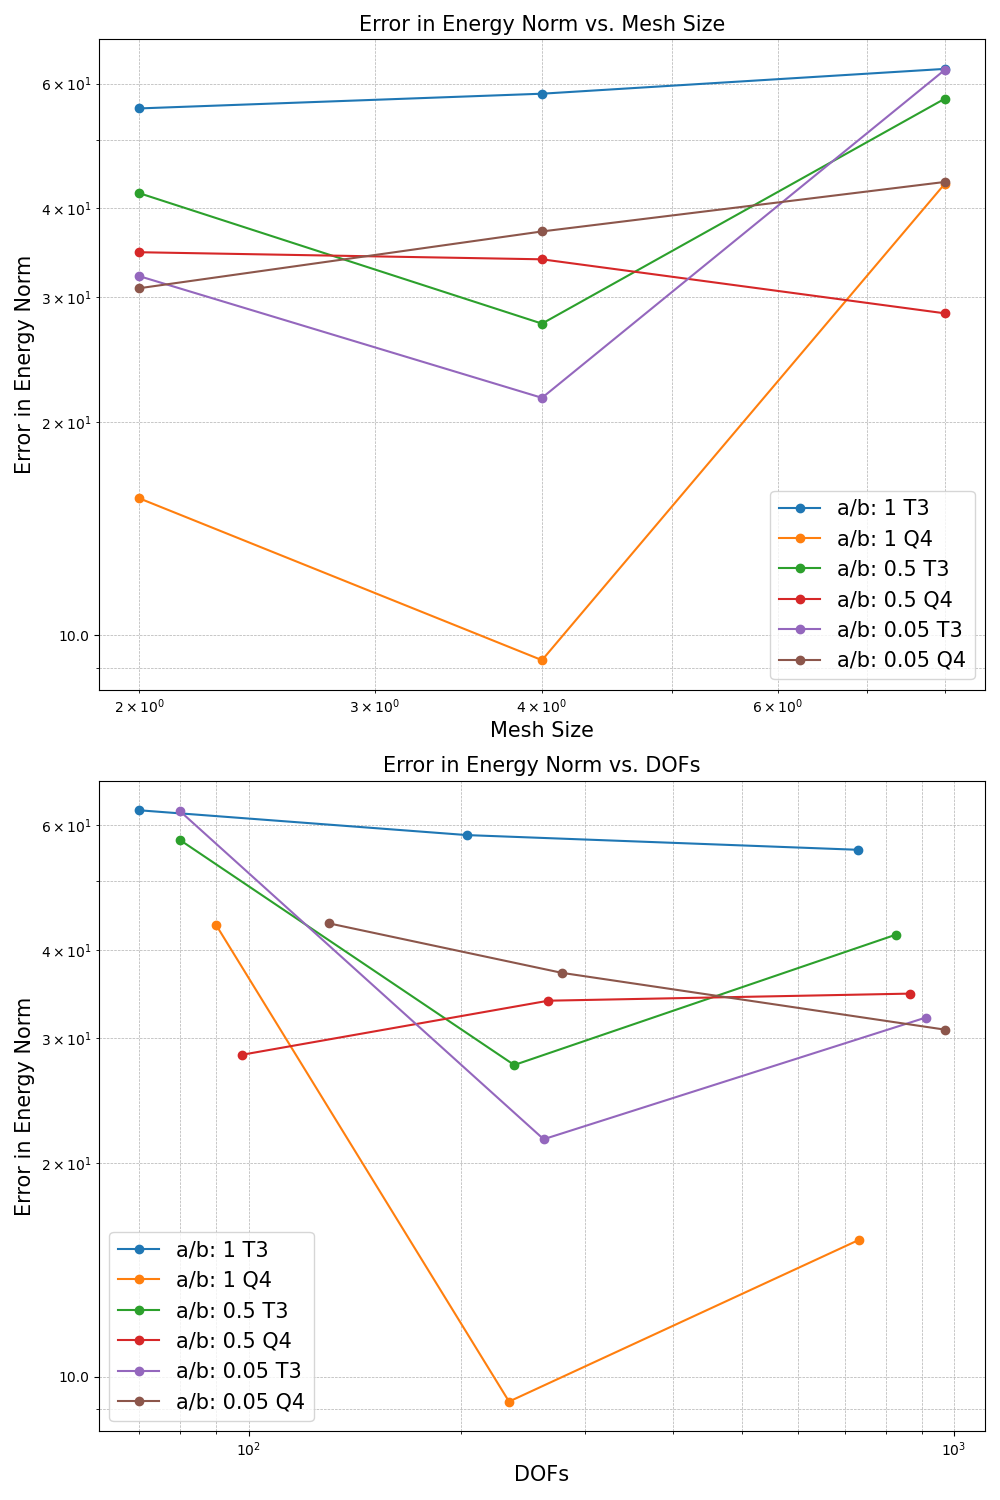
\includegraphics[width=1.\linewidth]{Q2_4/log_DOFs.png}
  \caption{Log-log plot of energy norm error versus DOFs.}
  \label{fig:logDOF_Q2_4}
\end{figure}
\begin{table}[ht]
  \centering
  \caption{Convergence Rates based on Mesh Size}
  \begin{tabular}{|c|c|c|}
  \hline
  \(a/b\) Ratio & Element Type & Convergence Rate \\
  \hline
  1 & T3 & 0.092621 \\
  1 & Q4 & 0.736803 \\
  0.5 & T3 & 0.221261 \\
  0.5 & Q4 & -0.143155 \\
  0.05 & T3 & 0.483199 \\
  0.05 & Q4 & 0.249004 \\
  \hline
  \end{tabular}
  \label{tab:convergenceRate_Meshsize}
\end{table}

\begin{table}[!ht]
    \centering
    \caption{Convergence Rates based on DOFs}
    \begin{tabular}{|c|c|c|}
    \hline
    \(a/b\) Ratio & Element Type & Convergence Rate\\
    \hline
    1 & T3 & -0.054701 \\
    1 & Q4 & -0.486695 \\
    0.5 & T3 & -0.131251 \\
    0.5 & Q4 & 0.091080 \\
    0.05 & T3 & -0.275252 \\
    0.05 & Q4 & -0.171758 \\
    \hline
    \end{tabular}
  \label{tab:convergenceRate_DOF}
\end{table}

Considering the fluctuation of the error is sensitive to the mesh size (the error reaches the lowest when the mesh size is 4), the convergence rates are calculated by the first point and the last point of the energy list.

The convergence rates for different elements with different a/b ratios concerning the mesh size and DOF are represented in Table.\ref{tab:convergenceRate_Meshsize} and Table.\ref{tab:convergenceRate_DOF}

\subsection*{Convergence Rates based on Mesh Size}

\begin{itemize}
    \item For T3 elements with \(a/b\) ratios of 1, 0.5, and 0.05, the observed convergence rates are 0.092621, 0.221261, and 0.483199, respectively.
    \item For Q4 elements with \(a/b\) ratios of 1, 0.5, and 0.05, the observed convergence rates are 0.736803, -0.143155, and 0.249004, respectively.
\end{itemize}

\subsection*{Convergence Rates based on DOFs}

\begin{itemize}
    \item For T3 elements with \(a/b\) ratios of 1, 0.5, and 0.05, the observed convergence rates are -0.054701, -0.131251, and -0.275252, respectively. 
    \item For Q4 elements with \(a/b\) ratios of 1, 0.5, and 0.05, the observed convergence rates are -0.486695, 0.091080, and -0.171758, respectively. 
\end{itemize}

It is observed that only for \(a/b = 1\) in T3 mesh and \(a/b = 0.5\) in Q4 mesh, the log-log plots appear to be linear. However, the convergence rates for all curves are lower than the expected theoretical values. The convergence rates of each mesh type in h-FEM in 2D are equal to the order of the interpolation polynomials over 2. Therefore, the experimentally observed convergence rates do not align with the theoretical predictions. However, from a trend perspective, it is observed that the error decreases as the mesh size gets smaller and also diminishes as the degrees of freedom (DOF) increase.

 
\subsection{Question 5}
Fig.\ref{fig:tri_1}, Fig.\ref{fig:quad_1}, Fig.\ref{fig:triangle_0.5}. Fig.\ref{fig:triangle_0.05} and Fig.\ref{fig:quad_0.05} represents the stress field of a/b ratie equal to {1, 0.5, 0.05}. For the Q4 element, the max stress value is selected by superconvergent patch recovery (SPR). The definition of the SPR method is in Appendix.\ref{Apdx:SPR}. The relative errors between the exact analytical solution and the FEM-obtained stress values are presented in Table~\ref{tab:stress_error}.

\begin{table}[ht]
\centering
\caption{Relative Errors Between Exact and FEM-obtained Stresses for Different a/b Ratios}
\label{tab:stress_error}
\begin{tabular}{cccc}
\toprule
a/b ratio & Error in \( \sigma_{x} \) (\%) & Error in \( \sigma_{y} \) (\%) \\
\midrule
1 & 57.33 & 805.00 \\
0.5 & 40.39 & 1130.77 \\
0.05 & 31.37 & 1820.00 \\
\bottomrule
\end{tabular}
\end{table}

Based on the relative error data, it is evident that the stress values have a higher level of relative error compared to the displacements. The relative errors in stress range from 31.37\% to 1820.00\%, while for displacements, they range from 6.83\% to 101.64\%. Therefore, in this particular case, the displacements appear to be more accurately predicted than the stresses.

\begin{figure}[!ht]
  \begin{subfigure}[c]{0.26\textwidth}
    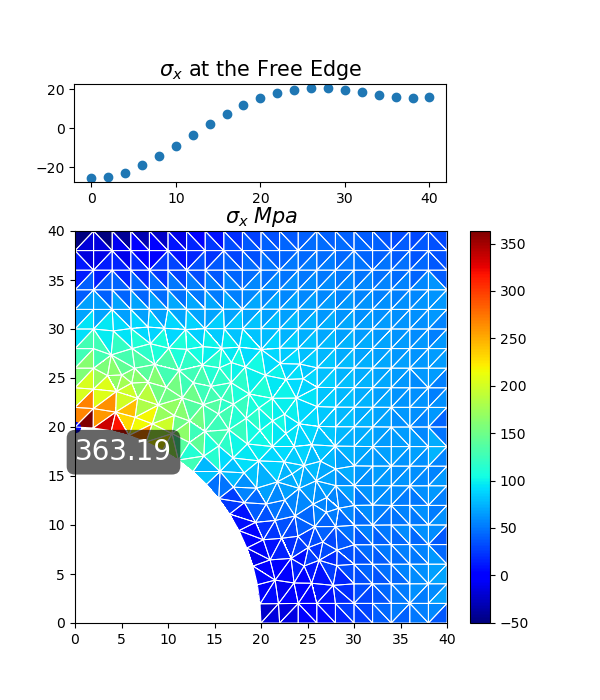
\includegraphics[width=1.\linewidth]{Q2_5/Q5_1_x_triangle.png}
    \caption{$\sigma_{xx}$}
    \label{fig:x_tri_1}
  \end{subfigure}%
  \begin{subfigure}[c]{0.26\textwidth}
    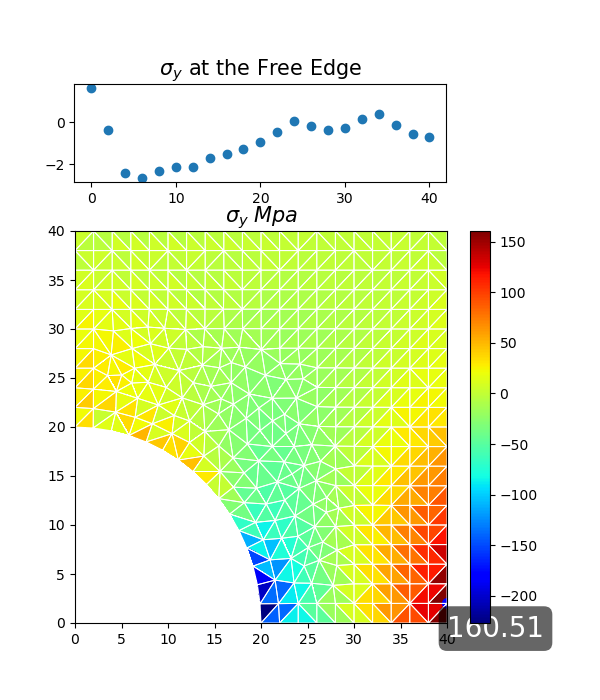
\includegraphics[width=1.\linewidth]{Q2_5/Q5_1_y_triangle.png}
    \caption{$\sigma_{yy}$ }
    \label{fig:y_tri_1}
  \end{subfigure}%
  \hfill
  \begin{subfigure}[c]{0.26\textwidth}
    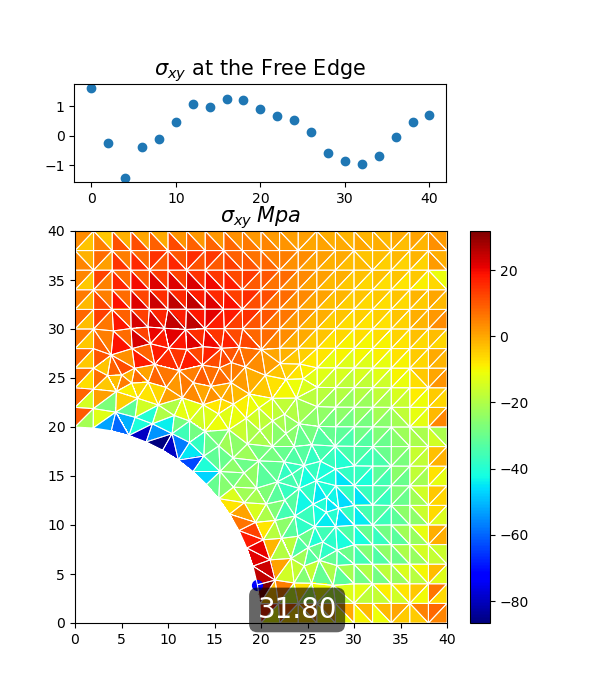
\includegraphics[width=1.\linewidth]{Q2_5/Q5_1_xy_triangle.png}
    \caption{$\sigma_{xy}$}
    \label{fig:xy_tri_1}
  \end{subfigure}%
  \begin{subfigure}[c]{0.26\textwidth}
    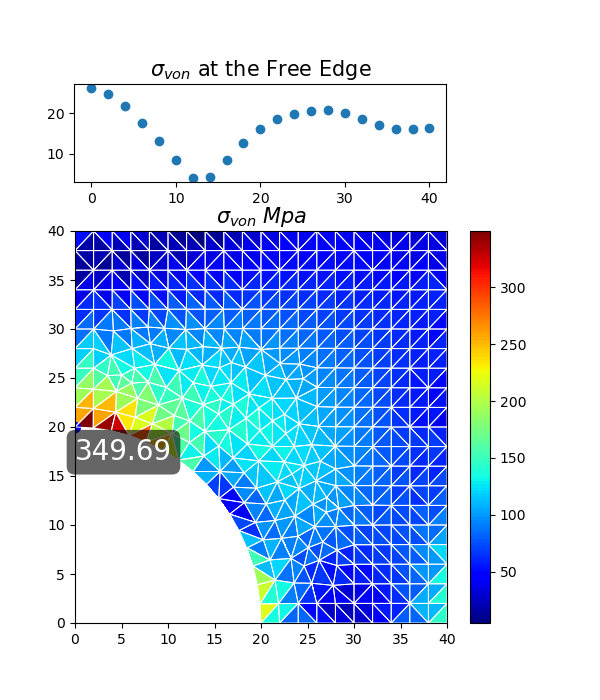
\includegraphics[width=1.\linewidth]{Q2_5/Q5_1_von_triangle.png}
    \caption{$\sigma_{von \, mise}$}
    \label{fig:von_tri_1}
  \end{subfigure}
  \caption{Stress fields for a/b=1 with T3 mesh.}
  \label{fig:tri_1}
\end{figure}

\begin{figure}[!ht]
  \begin{subfigure}[c]{0.26\textwidth}
    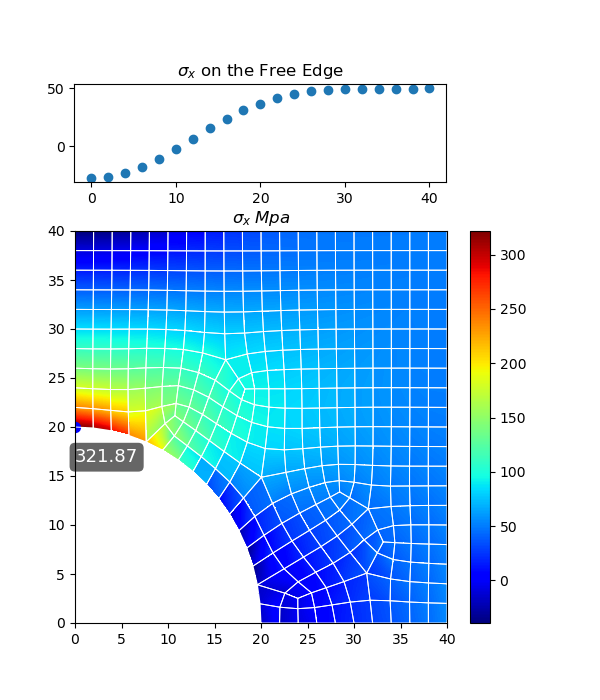
\includegraphics[width=1.\linewidth]{Q2_5/Q5_1_x_quad.png}
    \caption{$\sigma_{xx}$}
    \label{fig:x_quad}
  \end{subfigure}%  
  \begin{subfigure}[c]{0.26\textwidth}
    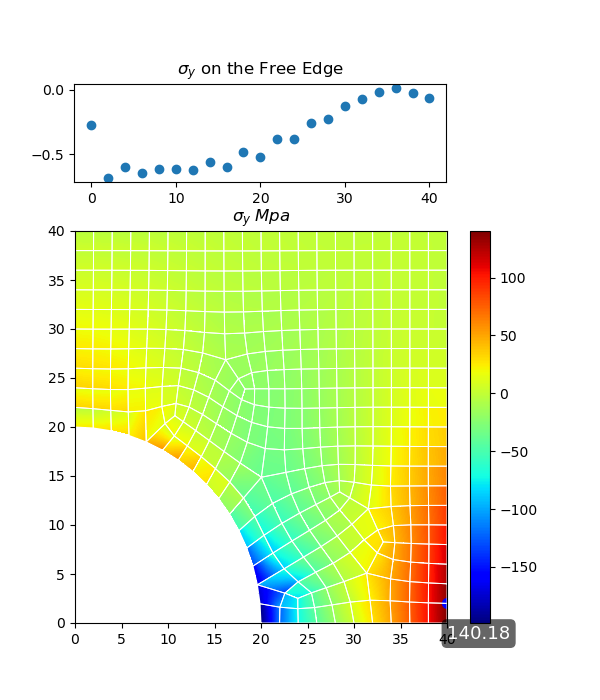
\includegraphics[width=1.\linewidth]{Q2_5/Q5_1_y_quad.png}
    \caption{$\sigma_{yy}$}
    \label{fig:y_quad}
  \end{subfigure}%  
  \hfill
  \begin{subfigure}[c]{0.26\textwidth}
    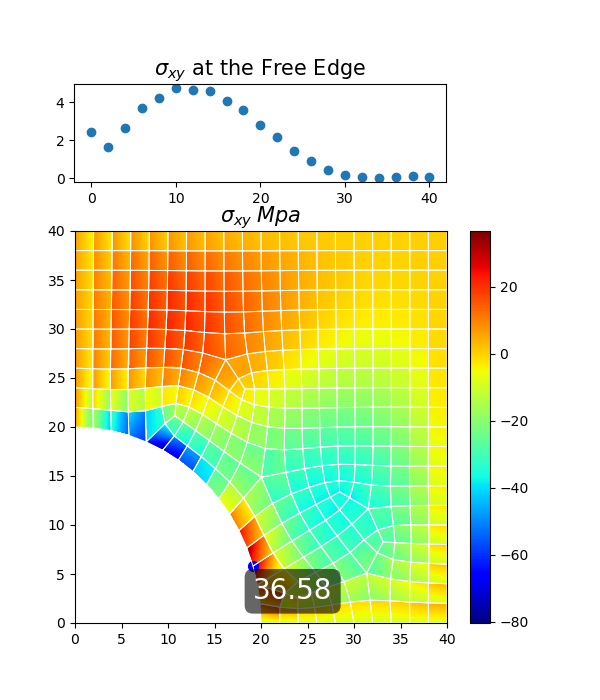
\includegraphics[width=1.\linewidth]{Q2_5/Q5_1_xy_quad.png}
    \caption{$\sigma_{xy}$}
    \label{fig:xy_quad}
  \end{subfigure}%  
  \begin{subfigure}[c]{0.26\textwidth}
    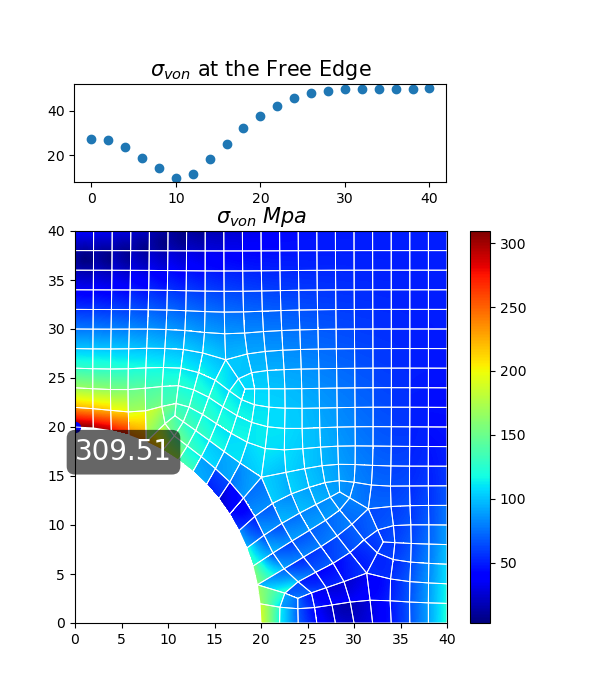
\includegraphics[width=1.\linewidth]{Q2_5/Q5_1_von_quad.png}
    \caption{$\sigma_{von \, mise}$}
    \label{fig:von_quad}
  \end{subfigure}
  \caption{Stress fields for a/b=1 with Q4 mesh.}
  \label{fig:quad_1}
\end{figure}


\begin{figure}[!ht]
  \begin{subfigure}[c]{0.26\textwidth}
    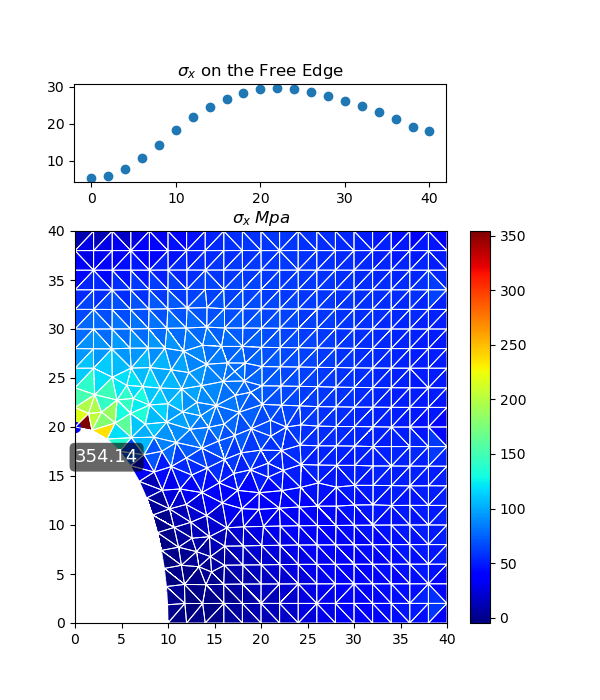
\includegraphics[width=1.\linewidth]{Q2_5/Q5_0.5_x_triangle.png}
    \caption{$\sigma_{xx}$}
    \label{fig:x_triangle_0.5}
  \end{subfigure}%  
  \begin{subfigure}[c]{0.26\textwidth}
    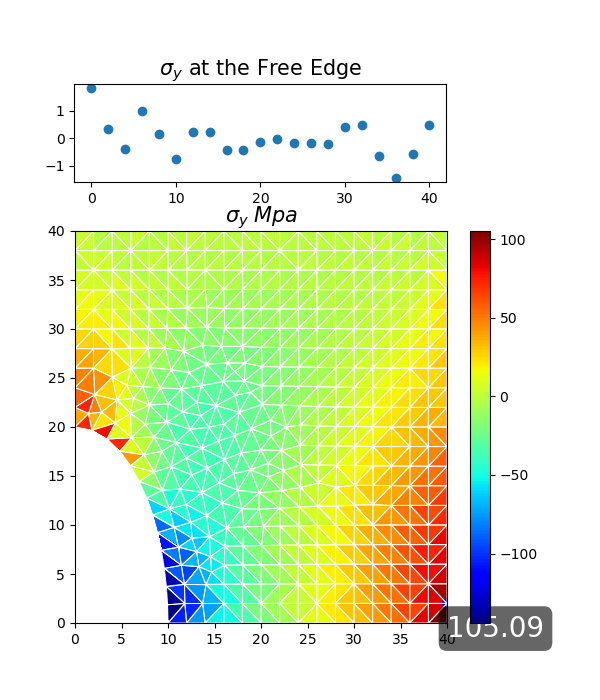
\includegraphics[width=1.\linewidth]{Q2_5/Q5_0.5_y_triangle.png}
    \caption{$\sigma_{yy}$}
    \label{fig:y_triangle_0.5}
  \end{subfigure}%  
  \hfill
  \begin{subfigure}[c]{0.26\textwidth}
    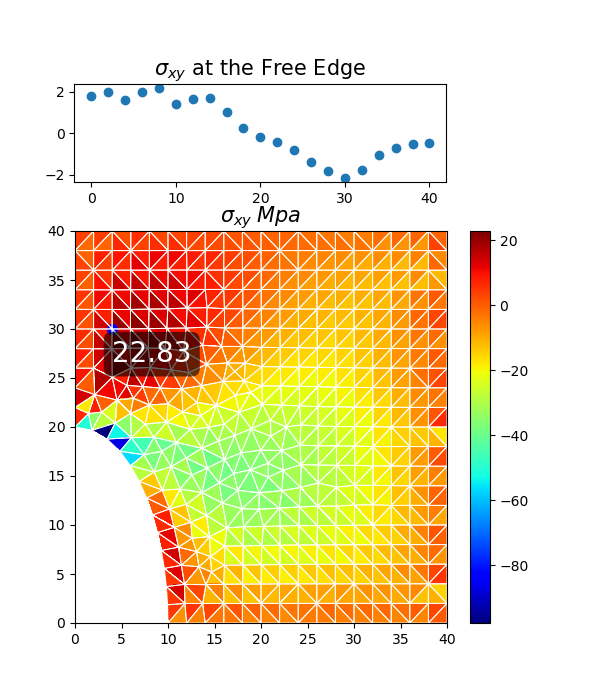
\includegraphics[width=1.\linewidth]{Q2_5/Q5_0.5_xy_triangle.png}
    \caption{$\sigma_{xy}$}
    \label{fig:xy_triangle_0.5}
  \end{subfigure}%  
  \begin{subfigure}[c]{0.26\textwidth}
    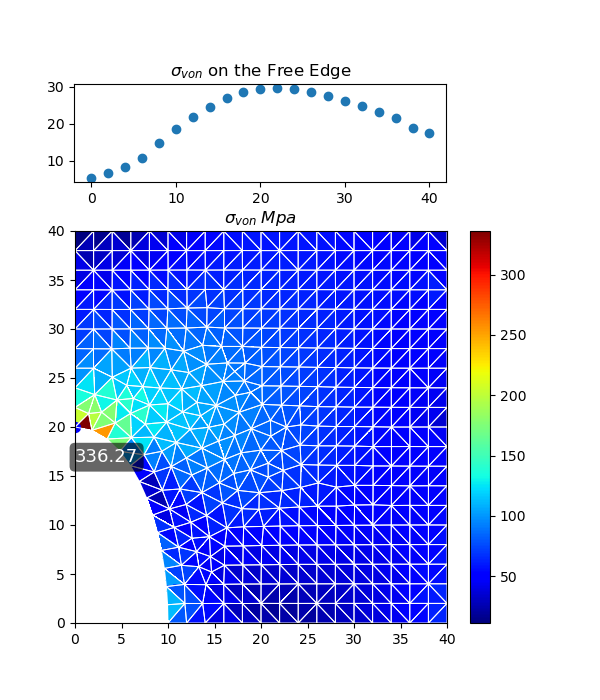
\includegraphics[width=1.\linewidth]{Q2_5/Q5_0.5_von_triangle.png}
    \caption{$\sigma_{von \, mise}$}
    \label{fig:von_triangle_0.5}
  \end{subfigure}
  \caption{Stress fields for a/b=0.5 with T3 mesh.}
  \label{fig:triangle_0.5}
\end{figure}

\begin{figure}[!ht]
  \begin{subfigure}[c]{0.26\textwidth}
    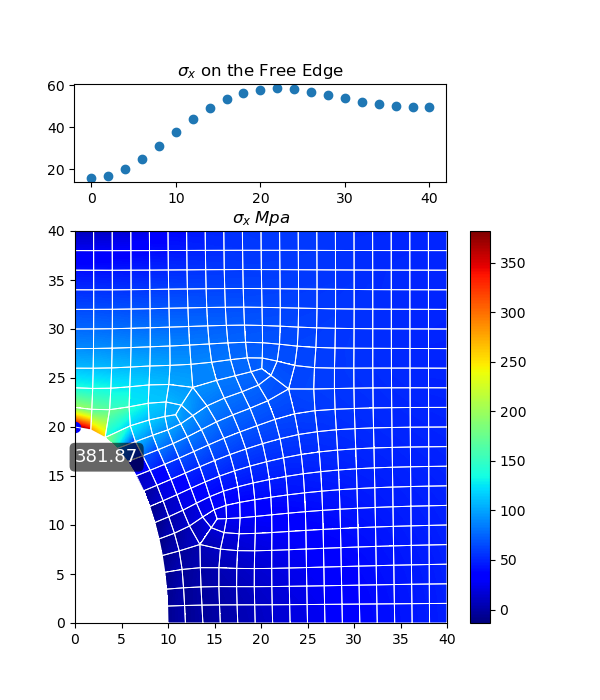
\includegraphics[width=1.\linewidth]{Q2_5/Q5_0.5_x_quad.png}
    \caption{$\sigma_{xx}$}
    \label{fig:x_quad_0.5}
  \end{subfigure}%  
  \begin{subfigure}[c]{0.26\textwidth}
    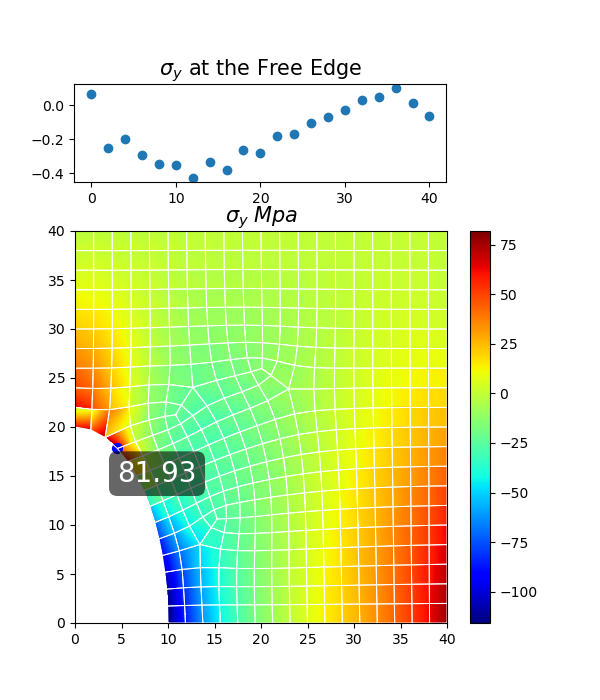
\includegraphics[width=1.\linewidth]{Q2_5/Q5_0.5_y_quad.png}
    \caption{$\sigma_{yy}$}
    \label{fig:y_quad_0.5}
  \end{subfigure}%  
  \hfill
  \begin{subfigure}[c]{0.26\textwidth}
    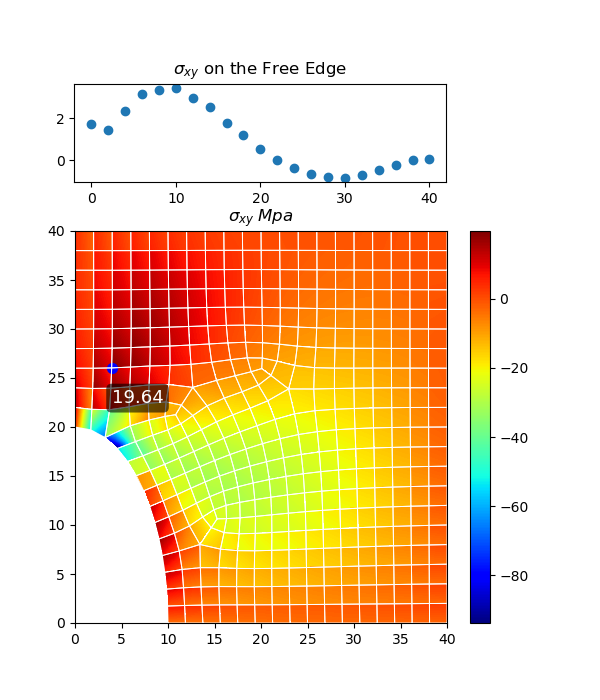
\includegraphics[width=1.\linewidth]{Q2_5/Q5_0.5_xy_quad.png}
    \caption{$\sigma_{xy}$}
    \label{fig:xy_quad_0.5}
  \end{subfigure}%  
  \begin{subfigure}[c]{0.26\textwidth}
    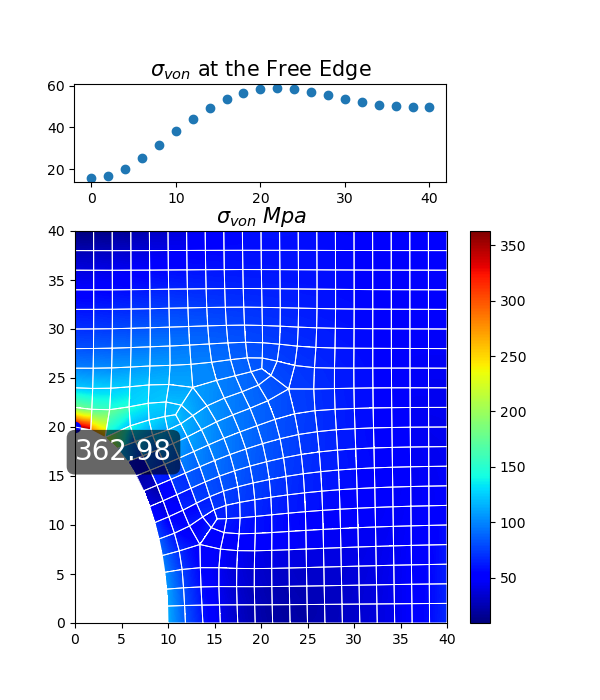
\includegraphics[width=1.\linewidth]{Q2_5/Q5_0.5_von_quad.png}
    \caption{$\sigma_{von \, mise}$}
    \label{fig:von_quad_0.5}
  \end{subfigure}
  \caption{Stress fields for a/b=0.5 with Q4 mesh.}
  \label{fig:quad_0.5}
\end{figure}

\begin{figure}[!ht]
  \begin{subfigure}[c]{0.26\textwidth}
    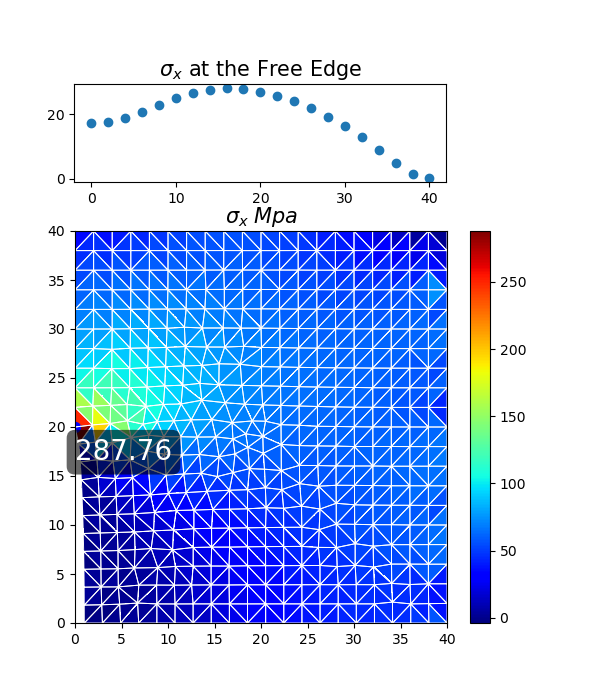
\includegraphics[width=1.\linewidth]{Q2_5/Q5_0.05_x_triangle.png}
    \caption{$\sigma_{xx}$}
    \label{fig:x_triangle_0.05}
  \end{subfigure}%  
  \begin{subfigure}[c]{0.26\textwidth}
    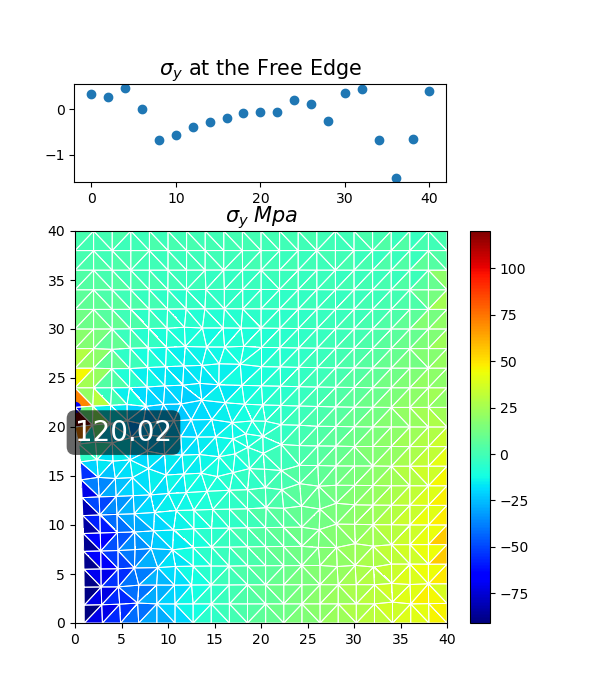
\includegraphics[width=1.\linewidth]{Q2_5/Q5_0.05_y_triangle.png}
    \caption{$\sigma_{yy}$}
    \label{fig:y_triangle_0.05}
  \end{subfigure}%  
  \hfill
  \begin{subfigure}[c]{0.26\textwidth}
    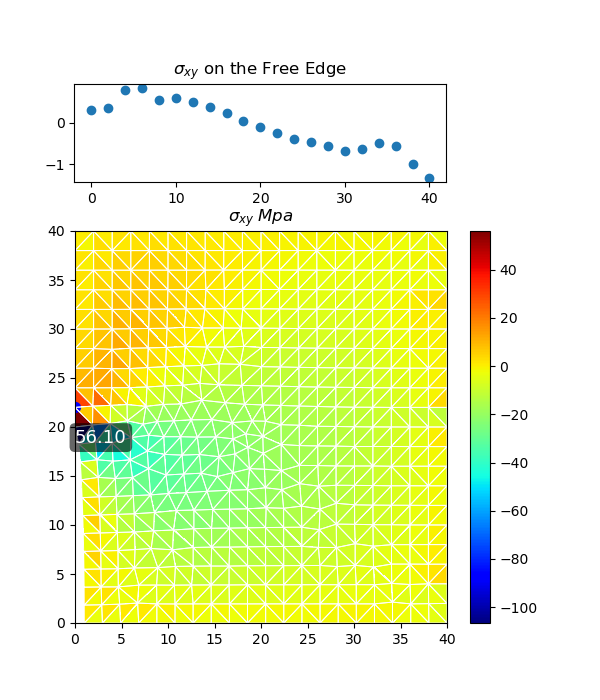
\includegraphics[width=1.\linewidth]{Q2_5/Q5_0.05_xy_triangle.png}
    \caption{$\sigma_{xy}$}
    \label{fig:xy_triangle_0.05}
  \end{subfigure}%  
  \begin{subfigure}[c]{0.26\textwidth}
    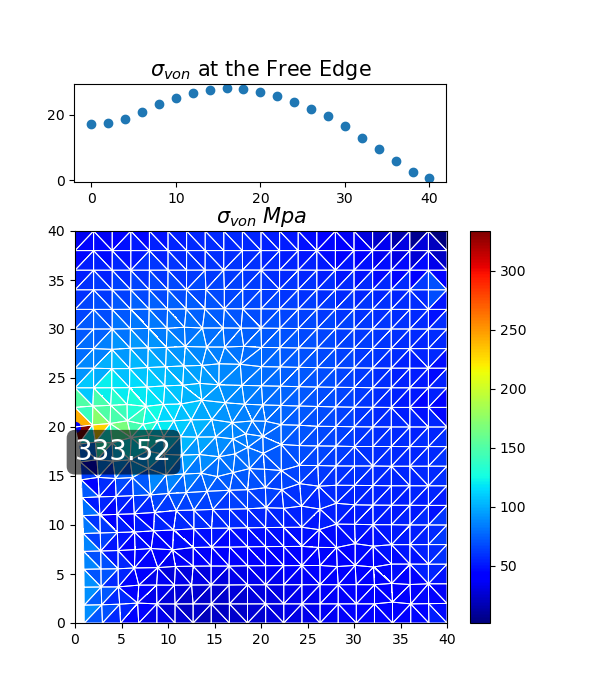
\includegraphics[width=1.\linewidth]{Q2_5/Q5_0.05_von_triangle.png}
    \caption{$\sigma_{von \, mise}$}
    \label{fig:von_triangle_0.05}
  \end{subfigure}
  \caption{Stress fields for a/b=0.05 with T3 mesh.}
  \label{fig:triangle_0.05}
\end{figure}

\begin{figure}[!ht]
  \begin{subfigure}[c]{0.26\textwidth}
    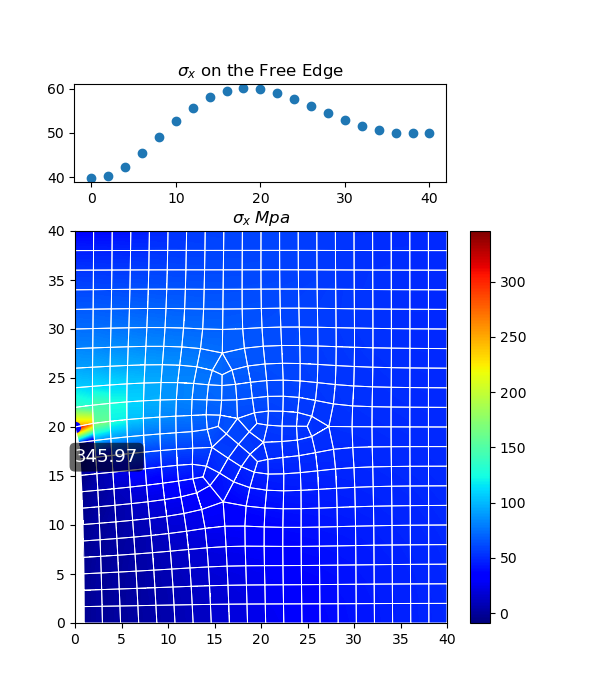
\includegraphics[width=1.\linewidth]{Q2_5/Q5_0.05_x_quad.png}
    \caption{$\sigma_{xx}$}
    \label{fig:x_quad_0.05}
  \end{subfigure}%  
  \begin{subfigure}[c]{0.26\textwidth}
    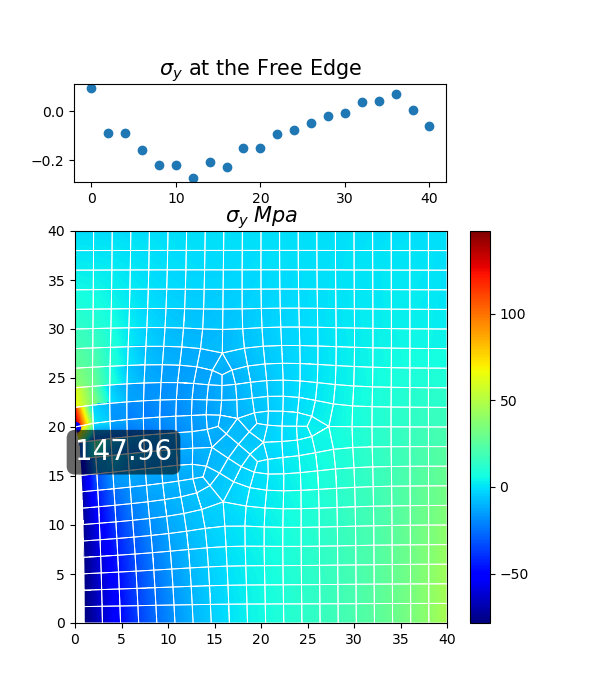
\includegraphics[width=1.\linewidth]{Q2_5/Q5_0.05_y_quad.png}
    \caption{$\sigma_{yy}$}
    \label{fig:y_quad_0.05}
  \end{subfigure}%  
  \hfill
  \begin{subfigure}[c]{0.26\textwidth}
    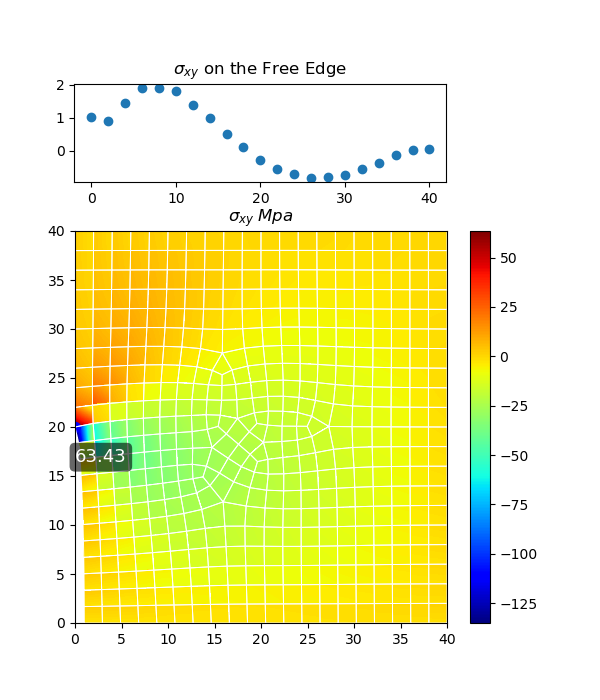
\includegraphics[width=1.\linewidth]{Q2_5/Q5_0.05_xy_quad.png}
    \caption{$\sigma_{xy}$}
    \label{fig:xy_quad_0.05}
  \end{subfigure}%  
  \begin{subfigure}[c]{0.26\textwidth}
    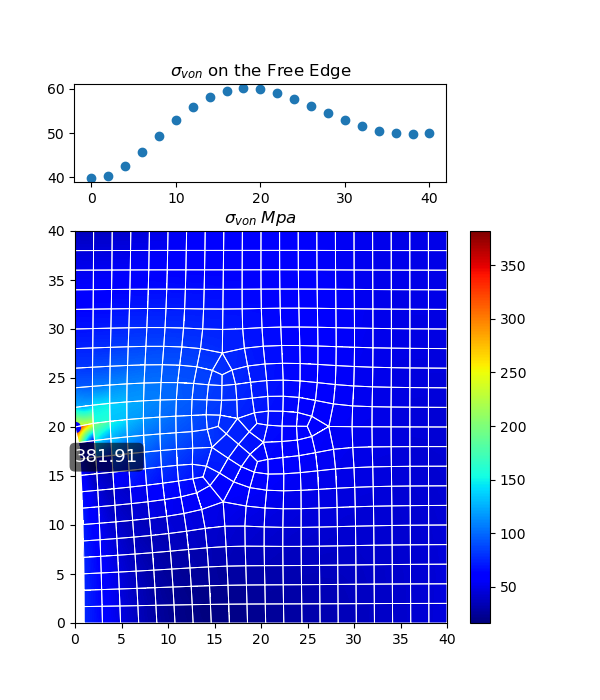
\includegraphics[width=1.\linewidth]{Q2_5/Q5_0.05_von_quad.png}
    \caption{$\sigma_{von \, mise}$}
    \label{fig:von_quad_0.05}
  \end{subfigure}
  \caption{Stress fields for a/b=0.05 with Q4 mesh.}
  \label{fig:quad_0.05}
\end{figure}

\subsection{Question 6}
The Table.\ref{tab:SCF} presents the stress concentration factors (SCF) for T3 and Q4 elements at different \(a/b\) ratios. It is evident that the experimentally observed SCFs are significantly different from the theoretical predictions (given by $K_c=1+2 \frac{b}{a}$).

\begin{itemize}
    \item For an \(a/b\) ratio of 1, both T3 and Q4 elements show SCFs (7.3 and 6.4, respectively) that are much higher than the theoretical value of 3. The average SCF is 6.85, which is more than twice the theoretical prediction.
    \item At an \(a/b\) ratio of 0.5, the SCFs for T3 and Q4 are 8.4 and 7.8, respectively, with an average of 8.1. This is also significantly higher than the theoretical value of 5.
    \item Interestingly, for an \(a/b\) ratio of 0.05, the SCFs are lower than the theoretical value. The SCFs for T3 and Q4 are 5.8 and 7, respectively, with an average of 6.4, which is far below the theoretical value of 41.
\end{itemize}

\begin{table}[!ht]
  \centering
  \caption{Stress Concentration Factors for T3 and Q4 Elements}
  \begin{tabular}{|c|c|c|c|c|}
  \hline
  \(a/b\) Ratio & T3 & Q4 & Average & Theory \\
  \hline
  1 & 7.3 & 6.4 & 6.85 & 3 \\
  0.5 & 8.4 & 7.8 & 8.1 & 5 \\
  0.05 & 5.8 & 7 & 6.4 & 41 \\
  \hline
  \end{tabular}
  \label{tab:SCF}
\end{table}

\subsection{Question 7}

The allowable stress values for the material under non-failing conditions at different a/b ratios are presented in the following Table.\ref{tab:criterion}. Von Mises criterion is selected as the criterion for the maximum allowable stress (shown in Appendix.\ref{Apdx:Von}).

\begin{table}[!ht]
\centering
\begin{tabular}{cccc}
\toprule
a/b  ratio & T3 & Q4 & Average \\
\midrule
1           & 30  & 33.9 & 31.95 \\
0.5         & 26.4& 28.9 & 27.65 \\
0.05        & 31.4& 27.3 & 29.35 \\
\bottomrule
\end{tabular}
\caption{Allowable stress values for different a/b ratios.}
\label{tab:criterion}
\end{table}


The table shows that the material has relatively consistent allowable stress values across different a/b ratios. Specifically, the average allowable stress is approximately 30, varying slightly from 27.65 to 31.95. This suggests that the material's allowable stress is not significantly influenced by the a/b ratio, indicating good material robustness under varying conditions.
\subsection{Question 8}

\subsection*{Strain Energy and Structural Integrity}

The calculated strain energy values for the three different \( a/b \) ratios indicate varying levels of structural integrity. For \( a/b = 1 \), the strain energy was highest, which suggests that the structure is energetically less stable when the hole is a circle. This could be attributed to higher localized stresses around the hole, making the structure more susceptible to energy accumulation.

For \( a/b = 0.5 \), the strain energy reduced compared to \( a/b = 1 \). This indicates that the structure becomes more stable as the hole becomes less elliptical. This could be due to a more uniform stress distribution around the hole, thus lowering the overall strain energy.

Interestingly, the lowest strain energy was observed for \( a/b = 0.05 \). This can be attributed to the shape of the hole, which is a very narrow ellipse at this ratio. In essence, the structure behaves almost like a solid plate with a crack, rather than a plate with a hole. The narrowness of the ellipse minimizes the global deformation, making the structure resemble a nearly intact plate.

\subsection*{Convergence Rates}

It was observed that the convergence rates deviated from the theoretical predictions, especially when \( a/b = 1 \). This could be attributed to the narrow ellipse at the center when \( a/b = 1 \), making the structure highly sensitive to mesh size. A fine mesh is needed for more accurate results, particularly in regions with strong gradients or stress concentrations.

\subsection*{Stress and Displacement Errors}

Both stress and displacement errors were considered. The stress errors were notably higher than those for displacements. For instance, stress errors ranged from 31.37\% to 1820.00\%, whereas displacement errors were between 6.83\% and 101.64\%. This suggests that the Finite Element model is more reliable for predicting displacements than for stresses.

\subsection*{Stress Concentration Factors (SCF)}

The SCFs deviated significantly from theoretical values, particularly at \( a/b = 1 \) and \( a/b = 0.5 \). This could be due to the coarse mesh used in the simulations. Also, the stress values at these concentrations were observed to increase as the mesh size decreased, possibly indicating the presence of a singularity. A singularity in this context means that the stress becomes infinite at a point, which is a known issue in the Finite Element Analysis of problems with sharp corners or re-entrant angles.

\subsection*{Mesh Sensitivity }

The observed sensitivity to mesh size, especially at \( a/b = 1 \), indicates that the simulations are less reliable in capturing the true behavior of the structure at this particular geometry. The abrupt stress values at points of stress concentration further support this observation. Therefore, the mesh size and element type play a crucial role in the simulation's reliability.

\subsection*{Validity of the Simulations}

While the study offers valuable insights into the performance of T3 and Q4 elements under various conditions, the findings should be interpreted with caution due to several limitations, such as mesh sensitivity and the potential for singularities. Furthermore, the observed convergence rate of the energy norm error deviates from the theoretical rate, particularly when the ratio a/b=0.3. For T3 elements in this case, the convergence rate exhibits a counterintuitive trend compared to other results. As such, a more refined definition of the mesh is warranted.



%------------------------------------------------

%------------------------------------------------

%----------------------------------------------------------------------------------------
%	REFERENCE LIST
% %----------------------------------------------------------------------------------------

\begin{thebibliography}{99} % Bibliography - this is intentionally simple in this template

\bibitem[Jin et al., 2014]{jin2014solution}
Jin, Xiaoqing and Wang, Zhanjiang and Zhou, Qinghua and Keer, Leon M and Wang, Qian (2014).
\newblock On the solution of an elliptical inhomogeneity in plane elasticity by the equivalent inclusion method.
\newblock {\em Journal of Elasticity}, 114:1--18.
 
\end{thebibliography}

%----------------------------------------------------------------------------------------

\hrule 
\newpage
%%\bibliographystyle{apacite}
%%\bibliography{sample}
%%\bibliographystyle{abbrv}

%%\bibliography{ref.bib} % the name of your .bib file without the extension
% Start the appendix
\appendix
\section{Defeinition of the 1-D Possion equation}
\label{Apdx:Q1}
The 1-D Poisson equation is given as:
\begin{equation}
-\frac{\mathrm{d}^2 u}{\mathrm{~d} x^2}=\frac{2\left(a+a^3 b(b-x+1)\right)}{\left(a^2 b^2+1\right)^2}
\end{equation}

with boundary conditions $(\mathrm{BCs}) u(0)=u(1)=0$, where $a$ is constant and $b=x-x_b$. The solution to this boundary value problem (BVP) is given by
\begin{equation}
u(x)=(1-x)\left(\arctan (a b)+\arctan \left(a x_b\right)\right)
\end{equation}



\section{Finite elements methods in 1-D main codes}
\label{Apdx:FEM_1D}
\begin{lstlisting}[language=Python, caption=Finite elements methods in 1-D main code]
  def FEM_1D(shape_class = Hierarchical, p = 3, num_elems = 3, domain = (0, 1),rhs_func = rhs_fn(a=50, xb=0.8), exact_func=exact_fn(0.5,0.8), BCs = (0, 0), verbose = False):
      N=6
      mesh = np.linspace(domain[0], domain[1], num_elems+1)
      ori_phi_phip = {'phis': [], 'phips': []}
      for elem in range(num_elems):
          scale = [mesh[elem], mesh[elem+1]]
          phis, phips = shape_class(scale, p)
          ori_phi_phip['phis'].append(phis)
          ori_phi_phip['phips'].append(phips)
  
  
      linear_phi_phip = {'phis': [], 'phips': []}  # Linear
      for elem in range(num_elems):
          linear_phis = []
          linear_phips = []
          for idx in range(len(ori_phi_phip['phis'][elem])):
              if ori_phi_phip['phis'][elem][idx].p < 2:
                  phi = ori_phi_phip['phis'][elem][idx]
                  phip = ori_phi_phip['phips'][elem][idx]
                  linear_phi_phip['phis'].append(phi)
                  linear_phi_phip['phips'].append(phip)
                  linear_phis.append(phi)
                  linear_phips.append(phip)
          linear_K_sub = np.zeros((len(linear_phips), len(linear_phips)))
          for indx, x in np.ndenumerate(linear_K_sub):
              linear_K_sub[indx] = G_integrate(
                  mul(linear_phips[indx[0]], linear_phips[indx[-1]]), N=6, scale=linear_phips[indx[0]].scale)
              if abs(linear_K_sub[indx]) < 1e-10:
                  linear_K_sub[indx] = 0
          linear_F_sub = np.zeros(len(linear_K_sub))
          for indx in range(len(linear_F_sub)):
              linear_F_sub[indx] = G_integrate(
                  mul(rhs_func, linear_phis[indx]), N=N, scale=linear_phis[indx].scale)
          if elem == 0:
              K = linear_K_sub
              F = linear_F_sub
          else:
              K = assemble(K, linear_K_sub)
              F = assemble(F, linear_F_sub)
              
      linear_num = len(F)
  
      nonlinear_phi_phip = {'phis': [], 'phips': []}
      for order in range(2, p+1):  # Non Linear
          for elem in range(num_elems):
              for idx in range(len(ori_phi_phip['phis'][elem])):
                  if (ori_phi_phip['phis'][elem][idx].p == order) or (ori_phi_phip['phips'][elem][idx].p == order):
                      nonlinear_phi = ori_phi_phip['phis'][elem][idx]
                      nonlinear_phip = ori_phi_phip['phips'][elem][idx]
                      nonlinear_phi_phip['phis'].append(nonlinear_phi)
                      nonlinear_phi_phip['phips'].append(nonlinear_phip)
                      nonlinear_K_sub = np.zeros((2, 2))
                      
                      nonlinear_K_sub[-1, -1] = G_integrate(mul(nonlinear_phip, nonlinear_phip),N=N, scale=nonlinear_phip.scale)
                      nonlinear_F_sub = np.zeros(2)
                      nonlinear_F_sub[-1] = G_integrate(mul(rhs_func, nonlinear_phi), N=N, scale=nonlinear_phi.scale)
  
                      K = assemble(K, nonlinear_K_sub)
                      F = assemble(F, nonlinear_F_sub)
                  else:
                      pass
                  
      # Applying boundary condition
  
      K[0, 1:] = 0.0 
      K[linear_num-1, :linear_num-1] = 0.0
      F[0] = BCs[0]* K[0, 0] 
      F[linear_num-1] = BCs[-1] * K[linear_num-1, linear_num-1]
  
      U = -la.solve(K, F)
      phi_phip = {'phis': [], 'phips': []}
      phi_phip['phis'] = joint_funcs(linear_phi_phip['phis']) + nonlinear_phi_phip['phis']
      phi_phip['phips'] = joint_funcs(linear_phi_phip['phips']) + nonlinear_phi_phip['phips']
      u_list = []
      for i in range(len(phi_phip['phis'])):
          u_list.append(mul(U[i], phi_phip['phis'][i]))
      uh = plus(u_list)
      if verbose == True:
          print(f"Shape class: {shape_class.__name__}, Number of elements: {num_elems}, Polynomial order:{p},  Domain: {domain}, Boundary conditions: {BCs}")
          x_data = np.linspace(domain[0], domain[1], 101)
          plt.plot(x_data, exact_func(x_data), label='Analytical solution')
          plt.plot(x_data, uh(x_data), label='FEM solution {} elements'.format(num_elems))
          for i in range(len(phi_phip['phis'])):
              func = phi_phip['phis'][i]
              plt.plot(x_data, U[i]*func(x_data))
          plt.legend()
          plt.show()
      eigenvalues = np.linalg.eigvals(K)
      cont_K = max(eigenvalues)/min(eigenvalues)
      return U, phi_phip, uh, cont_K
  
\end{lstlisting}

\section{Defeinition of the shape functions in 1D}
\label{Apdx:shape_1D}
\begin{lstlisting}[language=Python, caption=Defeinition of the shape functions in 1-D]
def Legendre(x=np.linspace(-1, 1, 100), p=5):

  if p == 0:
      return 1
  elif p == 1:
      return x

  else:
      return ((2*p-1)*x*Legendre(x, p-1)+(1-p)*Legendre(x, p-2))/p

class shape_function:
      def __init__(self, scale=[-1, 1]):
          self.scale = scale
          self.x_l = scale[0]
          self.x_r = scale[1]
          self.range = [-1, 1]
          
      def expression(self, x):
          return 1 - (x - self.x_l) / (self.x_r - self.x_l)
      
      def mapping(self, x):
          scale = self.scale
          range = self.range
          x_normalized = (x - scale[0]) / (scale[1] - scale[0])
          return range[0] + x_normalized * (range[1] - range[0])
  
      def __call__(self, x):
          x = np.asarray(x)  # convert x to a numpy array if it's not already
          expression_vectorized = np.vectorize(self.expression, otypes=['d'])
          return np.where((self.scale[0] <= x) & (x <= self.scale[-1]), expression_vectorized(x), 0)
      
class phi_func_l(shape_function):
  def __init__(self, scale, p):
      super().__init__(scale)
      self.p = p
      self.range = [0, 1]
  def expression(self, x):
      if self.p == 0:
          phi = 1-self.mapping(x)
      elif self.p == 1:
          phi = self.mapping(x) 
      else:
          raise AssertionError("p should be 0 or 1 in linear shape function, not{}".format(self.p))
      return phi
      
class phip_func_l(shape_function):
  def __init__(self, scale, p):
      super().__init__(scale)
      self.range = [0, 1]
      self.p = p
  def expression(self, x):
      scale_up = 1/(self.scale[1]-self.scale[0]) 
      
      if self.p == 0:
          phip =  np.zeros_like(self.mapping(x))-1
      elif self.p == 1:
          phip = np.zeros_like(self.mapping(x))+1
      else:
          raise AssertionError("p should be 0 or 1 in linear shape function, not{}".format(self.p))
      return phip*scale_up
  
class phi_func_q(shape_function):
  def __init__(self, scale, p):
      super().__init__(scale)
      self.range = [0, 1]
      self.p = p
  def expression(self, x):
      xx = self.mapping(x)
      if self.p == -1:
          phi = (xx-1)*(xx-0.5)*2
      elif self.p == 0:
          phi = -xx*(xx-1)*4
      elif self.p ==1:
          phi = xx*(xx-0.5)*2
      else:
          raise AssertionError("p should be -1, 0 or 1 in quadratic shape function, not{}".format(self.p))
      return phi
      
class phip_func_q(shape_function):
  def __init__(self, scale, p):
      super().__init__(scale)
      self.range = [0, 1]
      self.p = p
  def expression(self, x):
      scale_up = 1/(self.scale[1]-self.scale[0]) 
      xx = self.mapping(x)
      if self.p == -1:
          phip = 4*xx - 3.0
      elif self.p == 0:
          phip = 4-8*xx
      elif self.p ==1:
          phip = 4*xx - 1.0
      else:
          raise AssertionError("p should be -1, 0 or 1 in quadratic shape function, not{}".format(self.p))
      return phip*scale_up
  
class phi_func_h(shape_function):
  def __init__(self, scale, p):
      super().__init__(scale)
      self.p = p
  def expression(self, x):
      scale = self.scale
      i =self.p
      if i == 0:
          phi = (1-self.mapping(x))/2 
      elif i == 1:
          phi = (1+self.mapping(x))/2 
      else:
          phi = 1/np.sqrt(4*i-2)*(Legendre(self.mapping(x), i)-Legendre(self.mapping(x), i-2))
      return phi
      
class phip_func_h(shape_function):
  def __init__(self, scale, p):
      super().__init__(scale)
      self.p = p
  def expression(self, x):
      scale_up = 2/(self.scale[1]-self.scale[0]) 
      i =self.p
      
      if i == 0:
          phip =  np.zeros_like(self.mapping(x))-0.5
      elif i == 1:
          phip = np.zeros_like(self.mapping(x))+0.5
      else:
          phip = np.sqrt(i-1/2)*(Legendre(self.mapping(x), i-1))
      return phip*scale_up
  
def Hierarchical(scale, p):
  phis = []
  phips = []
  start=0
  
  for i in range(start, p+1):
      new_phi = phi_func_h(scale, i)
      new_phip = phip_func_h(scale,i)
      phis.append(new_phi)
      phips.append(new_phip)
  return phis, phips

def linear(scale, p):
  phis = []
  phips = []
  p = 1
  for i in range(p+1):
      new_phi = phi_func_l(scale, i)
      new_phip = phip_func_l(scale,i)
      phis.append(new_phi)
      phips.append(new_phip)
  return phis, phips

def quadratic(scale, p):
  phis = []
  phips = []
  p = 1
  for i in range(-1, p+1):
      new_phi = phi_func_q(scale, i)
      new_phip = phip_func_q(scale,i)
      phis.append(new_phi)
      phips.append(new_phip)
  return phis, phips
\end{lstlisting}

\section{Defeinition of Gaussian integrate in 1D}
\label{Apdx:Gaussian-1D}
\begin{lstlisting}[language=Python, caption=Defeinition of Gaussian integrate in 1D]
def G_integrate(u, N=3, scale=(0, 1)):
  N = N  
  a = scale[0] 
  b = scale[1]
  x, w = roots_legendre(N)

  xp = x*(b-a)/2+(b+a)/2
  wp = w*(b-a)/2

  s = 0
  for i in range(N):
      s += wp[i]*u(xp[i])
  return s
\end{lstlisting}

\section{Energy calculator in 1D}
\label{Apdx:energy-1D}
\begin{lstlisting}[language=Python, caption=Energy calculator in 1D]
def cal_energy(U_array, phi_phip_array):
  U_energy = 0
  u_prime_list = []
  scales = []
  for i in range(len(phi_phip_array['phis'])):
      u_prime = mul(U_array[i], phi_phip_array['phips'][i])
      u_prime_list.append(u_prime)
      scales.append(u_prime.scale)
  flat_scales = [item for sublist in scales for item in sublist]
  rounded_scales = [round(num, 5) for num in flat_scales]
  nodes = list(set(rounded_scales))
  mesh = np.linspace(min(nodes), max(nodes), len(nodes))
  for i in range(len(mesh)-1):
      scale = [mesh[i], mesh[i+1]]
      U_energy+=G_integrate(mul(plus(u_prime_list), plus(u_prime_list)),N=9, scale=scale)
  return U_energy/2
\end{lstlisting}

\section{A posteriori error estimate}
\label{Apdx:post}
\begin{lstlisting}[language=Python, caption=A posteriori error estimate]
def posterior_energy(energy_list_array, DOFs_array):
  if len(energy_list_array)<3:
      raise AssertionError("The value of energy should be greater than three!")
  elif len(energy_list_array)!= len(DOFs_array):
      raise AssertionError("The number of energy values should be equal to the number of DOFs!")
  def equation(U, U0, U1, U2, Q):
      return ((U-U0)/(U-U1) / ((U-U1)/(U-U2))**Q - 1)**2

  i = 0
  U_list = []
  while i+3 <= len(energy_list_array):
      U0, U1, U2 = energy_list_array[i:i+3]
      h0, h1, h2 = 1/np.sqrt(DOFs_array[i:i+3])
      # print(h0, h1, h2)
      N0, N1, N2 = DOFs_array[i:i+3]
      # Q = np.log((h0/h1))/np.log((h1/h2))
      Q = np.log((N1/N0))/np.log((N2/N1))
      initial_guess = np.mean(energy_list_array)
      # Use minimize
      U_solution = minimize(equation, initial_guess, args=(U0, U1, U2, Q)).x
      U_list.append(U_solution )
      i+=1
return np.mean(U_list)
\end{lstlisting}
  
\section{The definition of the traction-free hole in an infinite plate with different a/b ratios}
\label{Apdx:Q2}
\begin{figure}[!ht]
  \centering
  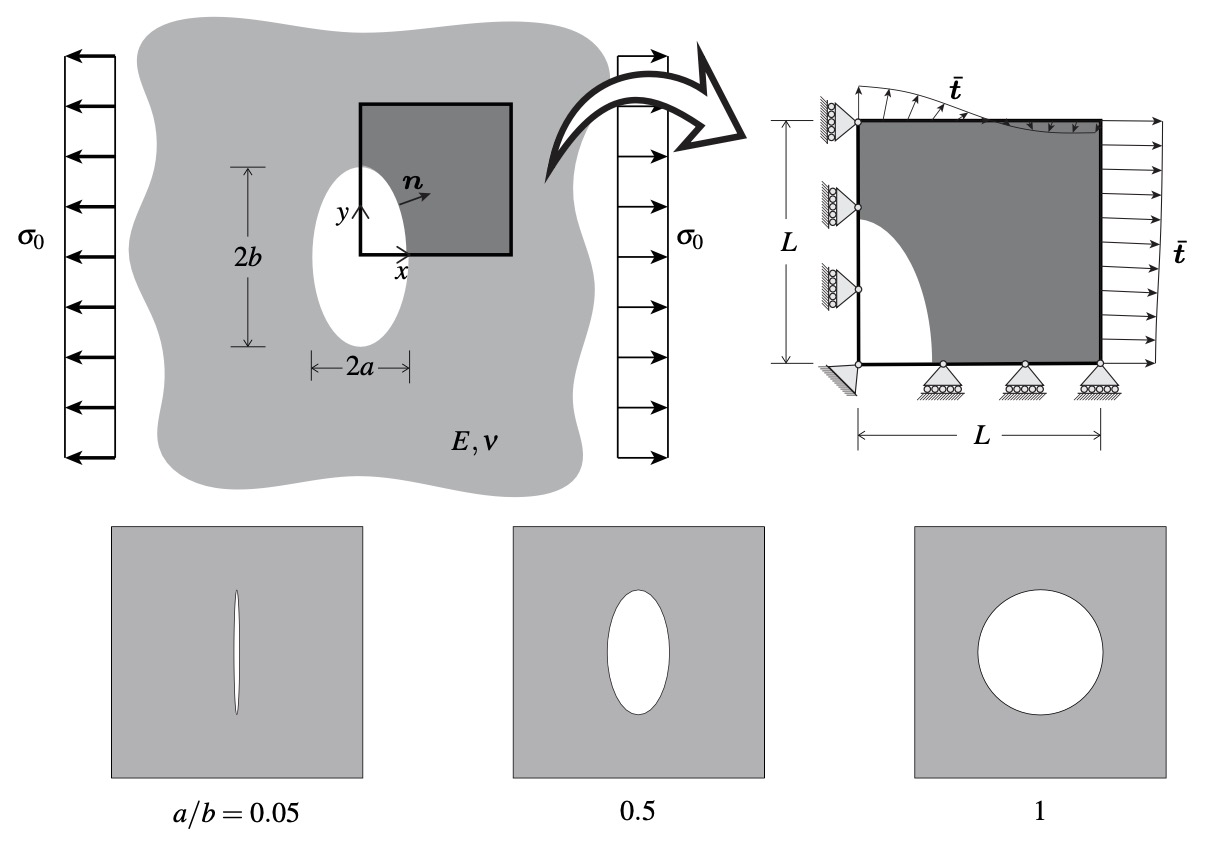
\includegraphics[width=1.\linewidth]{Q2_1/Q2.jpg}
  \caption{The definition of the traction-free hole in an infinite plate with different a/b ratios.}
  \label{fig:Q2}
\end{figure}

\section{Finite elements methods in 2D}
\label{Apdx:FEM_2D}
\begin{lstlisting}[language=Python, caption=Finite elements methods in 2D]
  def FEM(a_b, mesh_size, mesh_shape, GPN=2, show=False):
  Load_x = 50  # N/mm
  Load_y = 0  # N/mm
  nodes_coord,  element_nodes = create_mesh(a_b, mesh_shape, mesh_size)
  nodes_list = Boundary(nodes_coord, a_b)
  element_list = []
  if mesh_shape == 0:
      element_nodes = element_nodes.reshape(-1, 3)
  elif mesh_shape == 1:
      element_nodes = element_nodes.reshape(-1, 4)

  for ele_lst in element_nodes:
      this_nodes = [
          node for id in ele_lst for node in nodes_list if node.id == id]
      try:
          elem = Q4(this_nodes, GPN=GPN)
      except:
          elem = T3(this_nodes, GPN=GPN)
      elem.a_b = a_b
      element_list.append(elem)
  DOFs = 2*len(nodes_list)
  glo_K = np.zeros((DOFs, DOFs))
  glo_F = np.zeros(DOFs)

  for elem in element_list:  # Assemble Force vector
      loc_F = elem.F
      for i, node_i in enumerate(elem.nodes):
          global_dof = 2 * node_i.id
          # print(loc_F[2*i])
          if abs(node_i.xy[0]-40) < 1e-3:
              glo_F[global_dof] += Load_x * loc_F[2*i]
              # glo_F[global_dof] += Load_x * 1 
              glo_F[global_dof + 1] += Load_y * loc_F[2*i+1]

  for elem in element_list:  # Assemble Stiffness matrix
      loc_K = elem.K
      for i, node_i in enumerate(elem.nodes):
          for j, node_j in enumerate(elem.nodes):
              for dof_i in range(2):  
                  for dof_j in range(2):
                      global_dof_i = 2 * node_i.id + dof_i
                      global_dof_j = 2 * node_j.id + dof_j

                      glo_K[global_dof_i][global_dof_j] += loc_K[2 * i + dof_i][2*j + dof_j]
  for elem in element_list:  # Boundary condition

      for i, node_i in enumerate(elem.nodes):
          for dof_i in range(2):  
              global_dof_i = 2 * node_i.id + dof_i

              if node_i.BC[dof_i] == 1:

                  glo_K[global_dof_i, :] = 0
                  # glo_K[:, global_dof_i] = 0
                  glo_K[global_dof_i, global_dof_i] = 1e15  
                  glo_F[global_dof_i] = 0

  U = np.linalg.solve(glo_K, glo_F)
  for id in range(len(nodes_list)):
      displacement = np.array([U[id*2], U[id*2+1]])
      nodes_list[id].value = displacement

  if show == True:
      x_coords = [node.xy[0] for node in nodes_list]
      y_coords = [node.xy[1] for node in nodes_list]

      temperatures = [np.linalg.norm(node.value) for node in nodes_list]

      tri = []
      for c in element_nodes:
          tri.append([c[0], c[1], c[2]])
          try:
              tri.append([c[0], c[2], c[3]])
          except:
              pass

      plt.tricontourf(x_coords, y_coords, temperatures, triangles=tri,  levels=15, cmap=plt.cm.jet)
      plt.colorbar(label='Displacement in magnitude')
      plt.title('Displacements Distribution')

      plt.show()
  return U, nodes_coord, copy.deepcopy(element_list)


def draw(elements_list, dir='xy', type='disp', show = True):
  global_min = min([np.min([output(test_element(xy[0], xy[1], type), dir, type)
                      for xy in test_element.sample_points(refine)]) for test_element in elements_list])

  global_max = max([np.max([output(test_element(xy[0], xy[1], type), dir, type)
                      for xy in test_element.sample_points(refine)]) for test_element in elements_list])

  for test_element in elements_list:
      test_inputs = test_element.sample_points(refine)
      test_mapping = test_element.mapping(test_inputs)
      test_output = [output(test_element(xy[0], xy[1], type), dir, type)
                      for xy in test_inputs]
      test_x, test_y, test_z = grid_to_mat(test_mapping, test_output)
      # plt.scatter(test_mapping[:, 0], test_mapping[:, 1], s=1, c=test_output)
      plt.imshow(test_z, extent=(test_mapping[:, 0].min(),test_mapping[:, 0].max(), test_mapping[:, 1].min(), test_mapping[:, 1].max()), origin='lower', aspect='auto', interpolation='none',cmap='jet', vmin=global_min, vmax=global_max)
      vertices = test_element.vertices
      vertices = np.vstack([vertices, vertices[0]])
      vertices_x, vertices_y = zip(*vertices) 
      plt.plot(vertices_x, vertices_y,  color='white',
              linewidth=0.7)  

  plt.xlim(0, 40)
  plt.ylim(0, 40)
  # Display the color bar
  cbar = plt.colorbar()
  ticks = np.linspace(global_min, global_max, num=5)
  cbar.set_ticks(ticks)
  if type == 'disp':
      type_str = 'U'
  elif type == 'strain':
      type_str = '\\epsilon'
  elif type == 'stress':
      type_str = '\\sigma'
  dir_str = "{ %s }" % dir
  plt.title(rf"${type_str}_{dir_str}$")
  if show:
  plt.show()
\end{lstlisting}

\section{Defeinitions of shape functions for T3 and Q4 elements}
\label{Apdx:shape_2D}
\begin{lstlisting}[language=Python, caption=Defeinitions of shape functions for T3 and Q4 elements]
class shape_fns:
    def __init__(self, scale_x = [0, 1], scale_y = [0, 1], p=0):
        self.scale_x = scale_x
        self.scale_y = scale_y
        self.p = p
        
    def expression(self, xi, eta): 
        return 1-xi-eta

    def __call__(self, x=0, y=0):
        
        return  self.expression(x, y)


class T3_phi(shape_fns):
    def expression(self, xi, eta): 
        if self.p == 0:
             return xi 
        elif self.p == 1:
            return eta
        elif self.p == 2:
            return 1-xi-eta
        else:
            raise ValueError("p should be 0, 1 or 2 in T3 element shape functions, not {}".format(self.p))

        
class T3_phipx(shape_fns):
    def expression(self, xi=0, eta=0):
        if self.p == 0:
             return 1
        elif self.p == 1:
            return 0
        elif self.p == 2:
            return -1
        else:
            raise ValueError("p should be 0, 1 or 2 in T3 element shape functions, not {}".format(self.p))

class T3_phipy(shape_fns):
    def expression(self, xi=0, eta=0):
        if self.p == 0:
             return 0
        elif self.p == 1:
            return 1
        elif self.p == 2:
            return -1
        else:
            raise ValueError("p should be 0, 1 or 2 in T3 element shape functions, not {}".format(self.p))


class Q4_phi(shape_fns):
    def expression(self, xi=0, eta=0):
        if self.p == 0:
            return (xi-1)*(eta-1)/4
        elif self.p == 1:
            return (1 + xi) * (1 - eta)/4
        elif self.p == 2:
            return (1 + xi) * (1 + eta)/4
        elif self.p == 3:
            return (1 - xi) * (1 + eta)/4
        else:
            raise ValueError("p should be 0, 1, 2 or 3 in Q4 element shape functions, not {}".format(self.p))

class Q4_phipx(shape_fns):
    def expression(self, xi=0, eta=0):
        if self.p == 0:
             return (eta - 1)/4
        elif self.p == 1:
            return (1 - eta)/4
        elif self.p == 2:
            return (1 + eta)/4
        elif self.p == 3:
            return -(1 + eta)/4
        else:
            raise ValueError("p should be 0, 1, 2 or 3 in Q4 element shape functions, not {}".format(self.p))       


class Q4_phipy(shape_fns):
    def expression(self, xi=0, eta=0):
        if self.p == 0:
            return (xi - 1)/4
        elif self.p == 1:
            return -(xi + 1)/4
        elif self.p == 2:
            return (1 + xi)/4
        elif self.p == 3:
            return (1 - xi)/4
        else:
            raise ValueError("p should be 0, 1, 2 or 3 in Q4 element shape functions, not {}".format(self.p))
\end{lstlisting}

\section{Gaussian points in 2D}
\label{Apdx:Gaussian_2D}
\begin{lstlisting}[language=Python, caption=Gaussian points in 2D]
  def Gauss_points(element, order):
    if element.shape == 'quad':
        xi, wi = np.polynomial.legendre.leggauss(order)
        points = [(x, y) for x in xi for y in xi]
        weights = [wx * wy for wx in wi for wy in wi]
        
    elif element.shape == 'triangle':
        NGP_data = {
            1: {
                'points': np.array([(1/3, 1/3)]),
                'weights': np.array([1/2])
            },
            3: {
                'points': np.array([(1/6, 1/6), (2/3, 1/6), (1/6, 2/3)]),
                'weights': np.array([1/6, 1/6, 1/6])
            },
            4: {
                'points': np.array([(1/3, 1/3), (0.6, 0.2), (0.2, 0.6), (0.2, 0.2)]),
                'weights': np.array([-27/96, 25/96, 25/96, 25/96])
            }
        }
        if order == 2:
            order = 3
        points, weights = NGP_data[order]['points'], NGP_data[order]['weights']
    else:
        raise ValueError("Shape not supported")

    return points, weights 
\end{lstlisting}


\section{Von Mise stress}
\label{Apdx:Von}

The von Mises criterion, also known as the von Mises yield criterion or von Mises flow criterion, is a widely-used model for predicting the yielding behavior of ductile materials. Mathematically, it can be expressed as:
\subsection*{Von Mises Criterion According to the Implemented Code}

The von Mises stress criterion, as implemented in the provided Python code, is computed using the formula:

\[
\sigma_{\text{vM}} = \sqrt{\sigma_x^2 - \sigma_x \sigma_y + \sigma_y^2 + 3\tau_{xy}^2}
\]

Here, \( \sigma_x \) and \( \sigma_y \) are the normal stresses in the \( x \) and \( y \) directions, respectively, and \( \tau_{xy} \) is the shear stress in the \( xy \) plane.

The code for Von Mise stress is as follows:

\begin{lstlisting}[language=Python, caption=Von Mise stress]
  def Von_Mise(sigma_x, sigma_y, tau_xy):
        result = np.sqrt(sigma_x**2-sigma_x*sigma_y+sigma_y**2+3*tau_xy**2)
        return result
\end{lstlisting}



\section{Strain Energy in 2D}
\label{Apdx:energy}
\begin{lstlisting}[language=Python, caption=Strain energy in 2D]
def cal_energy(elements_list, GPN = 2):
  E = 200e3
  nu = 0.3
  D = E / (1 - nu**2)* np.array([
      [1, nu, 0],
      [nu, 1, 0],
      [0, 0, (1-nu)/2]
      ])
  energy = 0
  for elem in elements_list:
      elem_energy = 0
      points, Ws = Gauss_points(elem, GPN)
      loop = 0
      scale = 4 if elem.shape=="triangle" else 1
      for g in range(len(Ws)):
          xy = points[g]
          W = Ws[g]
          strain_list = elem(xy[0], xy[1], 'strain')
          dN = elem.gradshape(xy[0], xy[1])
          # J = jacobian(self.vertices, dN)
          J = np.dot(dN , elem.vertices)
          J_det = np.linalg.det(J)
          B = elem.B_matrix(J, dN)
          this_energy = 0.5 * W * strain_list.T @ D @ strain_list * J_det #* scale
          elem_energy += this_energy 
          loop+=1
      energy+=elem_energy
  return energy[0][0]
\end{lstlisting}


\section{Implementation of Superconvergent Patch Recovery}
\label{Apdx:SPR}
The Superconvergent Patch Recovery (SPR) method refines the stress distribution by extrapolating and averaging the stresses. The key steps can be mathematically represented as follows:

\begin{enumerate}
    \item \textbf{Stress at Gauss Points}: The stress \( \sigma_{\text{Gauss}} \) is initially calculated at the Gauss points of each finite element.
    \[
    \sigma_{\text{Gauss}} = C : \varepsilon_{\text{Gauss}}
    \]
    where \( C \) is the material stiffness matrix, and \( \varepsilon_{\text{Gauss}} \) is the strain at the Gauss points.

    \item \textbf{Extrapolation to Nodes}: The stress is then extrapolated to the nodes \( N \) of each element using shape functions \( N_i \).
    \[
    \sigma_{\text{Node}} = \sum_{i=1}^{n} N_i \sigma_{\text{Gauss}, i}
    \]
    where \( n \) is the number of Gauss points.

    \item \textbf{Averaging at Nodes}: Finally, the nodal stresses are averaged across adjacent elements to get a smoother stress distribution \( \sigma_{\text{avg}} \).
    \[
    \sigma_{\text{avg}} = \frac{1}{m} \sum_{j=1}^{m} \sigma_{\text{Node}, j}
    \]
    where \( m \) is the number of nodes shared by adjacent elements.
\end{enumerate}



 
\end{document}
